\documentclass{Academic}
\addbibresource{references.bib}
\usepackage{tikz}
\usetikzlibrary{positioning,arrows.meta,shapes.geometric}
\usepackage{tabularx}
\usepackage{placeins}
\usepackage{csquotes}

% Reduce LaTeX float-to-text spacing
\setlength{\textfloatsep}{10pt plus 2pt minus 4pt}
\setlength{\floatsep}{8pt plus 2pt minus 2pt}
\setlength{\intextsep}{8pt plus 2pt minus 2pt}
% Float pages: push figure to top rather than centering it
\makeatletter\setlength{\@fptop}{0pt}\makeatother
\setlength{\abovecaptionskip}{4pt}
\setlength{\belowcaptionskip}{0pt}
\renewcommand{\topfraction}{0.9}
\renewcommand{\bottomfraction}{0.85}
\renewcommand{\textfraction}{0.07}
\renewcommand{\floatpagefraction}{0.85}
\setcounter{topnumber}{3}
\setcounter{bottomnumber}{2}
\setcounter{totalnumber}{5}
\captionsetup{justification=raggedright, singlelinecheck=false}
% Prevent widows/orphans but allow mid-paragraph page breaks
\widowpenalty=10000
\clubpenalty=10000
\brokenpenalty=10000

% Pipeline stage macro: #1=image file  #2=bg colour  #3=title  #4=bullet lines
\newcommand{\pstage}[4]{%
  \noindent
  \begin{tabular}{@{}p{0.34\linewidth}@{\hspace{0.03\linewidth}}c@{\hspace{0.03\linewidth}}p{0.54\linewidth}@{}}
    \colorbox{#2}{\parbox{\dimexpr\linewidth-2\fboxsep}{%
      \raggedright\vspace{3pt}%
      \textbf{#3}\\[3pt]%
      \footnotesize #4%
      \vspace{3pt}}} &
    $\rightarrow$ &
    \centering
    \IfFileExists{figures/#1}%
      {\includegraphics[height=3.2cm,width=\linewidth,keepaspectratio]{figures/#1}}%
      {\rule{0pt}{3.2cm}} \\
  \end{tabular}%
}
\newcommand{\psarrow}{%
  \par\vspace{0.1cm}\hfill{\large$\Big\downarrow$}\hfill\par\vspace{0.1cm}}
% Pre-defined stage colours (avoids fragile inline-mixing in \newcommand args)
\AtBeginDocument{%
  \colorlet{stageGray}{gray!18}%
  \colorlet{stageGreen}{green!12}%
  \colorlet{stageOrange}{orange!15}%
  \colorlet{stageBlue}{blue!12}%
  \colorlet{stagePurple}{purple!10}%
  \colorlet{stagePlaceholder}{black!8}%
}


\begin{document}
%TC:ignore
\myabstract{Blood collection tubes are among the most widely used single-use medical plastics: a large hospital processes tens of thousands per day, yet virtually all are incinerated alongside hazardous clinical waste. Manual sorting at scale poses unacceptable infection risk to workers, motivating an automated circular economy pipeline in which tubes are \emph{segregated} by cap type, \emph{opened}, \emph{cleaned} and \emph{sterilised}, then returned to \emph{reuse} or single-polymer material recovery. The tubes in this study are unused, uncontaminated specimens captured in a controlled laboratory setting. Their partially transparent, specularly reflective surfaces make colour-based classification less reliable under varying clinical lighting---a central motivation for the RGB-D (colour plus depth) approach taken in this work.

The target deployment is a conveyor-belt sorter presenting one tube at a time to an overhead camera, with a pneumatic air-jet directing each tube to the correct recovery stream. The system targets sub-25\,ms per-frame latency; all experiments are performed on static images in a controlled laboratory environment, establishing baselines before dynamic validation at belt speed.

A dataset of 3\,000 paired RGB and depth images was captured with an Intel RealSense D415 depth camera and annotated across four cap-closure classes (Universal, Push-on, Screwcap, Other) using SAM~2-assisted polygon labelling on Roboflow. Five YOLO-family instance segmentation models were evaluated across RGB, RGBD, and depth-only input modalities. Adding a depth channel to a compact 2.8\,M-parameter model (YOLO11n-RGBD, mask mAP\textsubscript{50--95}\,=\,0.929) outperformed a network ten times larger trained on RGB alone (YOLOv8m-seg, 0.905); YOLO26n-seg delivered the best speed--accuracy trade-off at 23.1\,ms per frame. A depth-only model reached 0.804, confirming that tube geometry is discriminative and robust to the reflective and transparent surfaces that challenge colour-based classification. A live inference pipeline demonstrates classification at 30--45\,fps, ready for integration with the conveyor-belt sorting hardware.

}
\renewcommand{\myTitle}{High-Speed RGB-D Segmentation for Automated Medical Tube Segregation}
\renewcommand{\MyAuthor}{Tadeas Horn}
\renewcommand{\MyDepartment}{Department of Mechanical Engineering}
\renewcommand{\ID}{3035743}
\renewcommand{\Keywords}{Instance Segmentation, Medical Tubes, YOLO, RGB-D Fusion, Circular Economy}
\renewcommand{\MySupervisor}{Shiv Ashutosh Katiyar}
\maketitle
\onehalfspacing
\setlength{\emergencystretch}{3em}
\raggedbottom
%TC:endignore

%%====================================================================
\section{Introduction}
\label{sec:introduction}
%%====================================================================

Every large hospital processes thousands of blood collection tubes each day; virtually all are incinerated. In England alone, healthcare generates an estimated 156,000\,tonnes of clinical waste annually, the majority of which is non-hazardous and potentially recoverable~\supercite{who2024healthcare,windfeld2015medical}. The COVID-19 pandemic highlighted the scale: over 27,000\,tonnes of personal protective equipment were distributed in England within six months~\supercite{rizan2021environmental}. Polypropylene and polyethylene tubes, which make up the bulk of blood collection containers, can be recovered and reused as material at rates of 70--80\% when properly segregated by type~\supercite{lee2004medical,geyer2017plastics}; cap removal further enables component-level recovery of both body and closure materials. Realising this potential requires a structured circular pathway: tubes are first \emph{segregated} by closure type, then \emph{opened} to separate cap from body, before being \emph{cleaned} and \emph{sterilised} to decontaminate surfaces, and finally returned to direct \emph{reuse} or directed to single-polymer material recovery~\supercite{lee2004medical}---every downstream step depends on accurate prior classification. Direct reuse at the top of this hierarchy, returning sterilised sorted tubes to secondary service, preserves the full embodied manufacturing value of each item and avoids the energy cost of re-melting. The NHS commitment to net-zero emissions by 2040~\supercite{nhs2022netzero} provides strong institutional motivation to divert these materials from incineration.

Manual sorting is not only labour-intensive and error-prone but is fundamentally unsafe at scale: even capped and nominally sealed tubes carry contaminated exterior surfaces from centrifuge and processing environments, exposing workers to unacceptable biological-sample risk~\supercite{chartier2014safe}. Automated classification is therefore a safety necessity, not merely a convenience. Computer vision offers a scalable alternative. The YOLO (You Only Look Once) family of detectors~\supercite{redmon2016yolo} enables real-time object detection by treating localisation as a single regression problem. Subsequent versions built on the original architecture: YOLOv8~\supercite{jocher2023yolov8} added a decoupled head for separate classification and regression branches, YOLO11~\supercite{jocher2024yolo11} improved feature extraction efficiency for mobile deployment, and YOLO26 introduced end-to-end NMS-free inference. Instance segmentation extends detection by predicting pixel-level masks for each detected object, providing precise spatial boundaries rather than approximate bounding boxes. Mask~R-CNN~\supercite{he2017maskrcnn} established the two-stage approach, while YOLO-seg variants achieve similar mask quality at much higher throughput by sharing the detection backbone for mask generation.

For a tube-sorting application, instance masks offer three concrete advantages over bounding-box detection. First, per-tube mask centroids and principal axes will guide a downstream air-jet actuator to the correct position on the tube, a capability that becomes critical once the system is deployed on a moving belt. Second, pixel-level boundaries allow shape metrics---cap area ratio, tube elongation, and width-to-length profile---to be computed directly from the mask, providing discriminative features for classes whose bounding boxes overlap in size; Screwcap and Push-on tubes, for example, produce similar axis-aligned box dimensions but differ markedly in mask shape. Third, component-level disassembly requires pixel-level knowledge of where the cap meets the tube shaft; bounding boxes cannot provide this, and the present work lays the mask-level foundation for that downstream step.

Depth sensing provides additional geometric information that can improve object detection and classification. The Intel RealSense D400 series uses active infrared stereo to generate dense depth maps at video frame rates~\supercite{keselman2017realsense}. The D415 model projects a structured infrared pattern onto the scene and computes disparity between left and right infrared cameras to triangulate depth at each pixel, achieving sub-millimetre precision at short range. Previous work has shown that combining RGB and depth channels improves recognition under occlusion and lighting variation~\supercite{eitel2015rgbd}; the present work adopts direct normalisation, appending depth as a normalised 8-bit channel without additional preprocessing dependencies. Depth is especially relevant for medical tubes because their transparent and reflective plastic surfaces can make purely colour-based classifiers less reliable---specular highlights, colour ambiguity under varying lighting, and transparent tube bodies are all conditions that depth measurements handle robustly. These considerations motivate the inclusion of depth-channel training in this project, where paired RGB--depth data are fused into four-channel RGB-D inputs and also evaluated as depth-only single-channel models. Depth also enables metric localisation: applying the camera's intrinsic parameters to each mask centroid would give an air-jet controller the belt position needed to trigger precisely; this capability is reserved for future integration.

This project extends Jessiah Buamah's digital-twin framework, which used reinforcement learning to control pneumatic air jets on a simulated conveyor belt but achieved limited accuracy due to small synthetic training data. The present work addresses this by building a real-image annotated dataset and comparing five YOLO segmentation architectures across RGB, RGB-D, and depth-only modalities. No published study has applied instance segmentation to medical tube classification with paired depth data. Three contributions distinguish this work: a real-image RGB-D instance segmentation dataset for clinical blood collection tubes; explicit linking of cap closure type to disassembly route and material stream; and empirical demonstration that depth fusion is a more efficient path to high accuracy than scaling the model.

This work provides the vision component of a larger integrated system: an inclined feed channel on the conveyor belt presents one tube at a time to the overhead camera, guaranteeing single-tube presentation and matching the one-tube-per-session data collection protocol used throughout. The production-line target uses the SR2000 industrial scanning head, which demands sub-25\,ms classification latency; all experiments reported here are performed on static images in a controlled laboratory environment, establishing accuracy and speed baselines before dynamic testing at belt speed once the conveyor hardware is commissioned. The specific objectives are: (1)~to collect and annotate a dataset of single-use medical tube images captured with an Intel RealSense D415 depth camera; (2)~to train and evaluate YOLO-family models for four-class instance segmentation across RGB, RGB-D, and depth-only modalities; and (3)~to demonstrate real-time inference as a proof-of-concept for integration with the downstream conveyor-belt sorting hardware. Two research questions frame the experimental evaluation: \textbf{RQ1}---Is cap-closure type a sufficient basis for automated disassembly and material-stream decisions?---and \textbf{RQ2}---Can adding a depth channel to a compact segmentation model match or exceed a larger RGB-only model while maintaining real-time speed? Training and evaluation used unused, uncontaminated specimens only; post-use testing is reserved for future work. \Cref{fig:pipeline_flow} summarises the end-to-end pipeline adopted in this work.

%%====================================================================
\section{Literature Review}
\label{sec:litreview}
%%====================================================================

\begin{figure}[p]
\vspace*{\fill}
\centering
  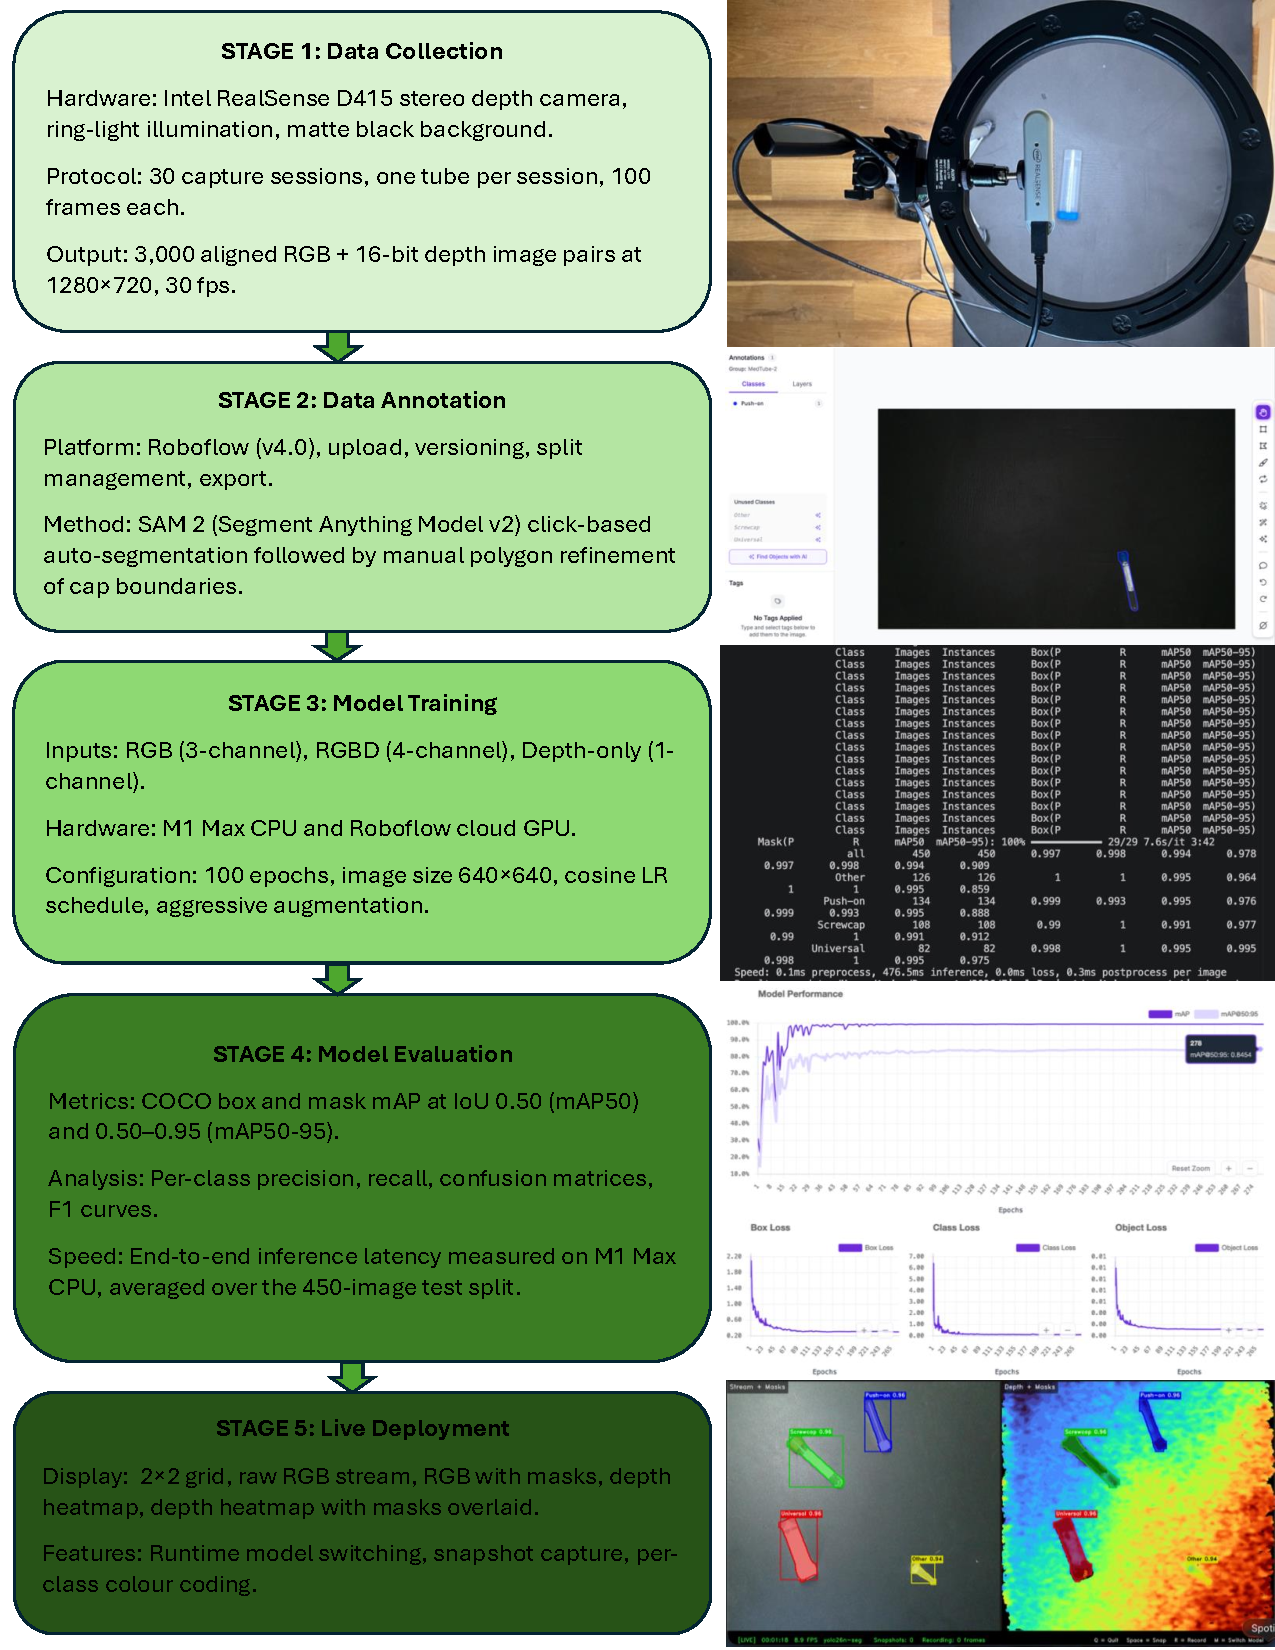
\includegraphics[width=\linewidth,height=0.88\textheight,keepaspectratio]{figures/FYP_Figure_1.pdf}
  \caption{End-to-end project pipeline. Each stage shows the pipeline step with a representative screenshot. Top to bottom: Data Collection, Data Annotation, Model Training, Model Evaluation, Live Deployment.}
  \label{fig:pipeline_flow}
\vspace*{\fill}
\end{figure}

\subsection{YOLO-based instance segmentation}
YOLO architectures~\supercite{redmon2016yolo} achieve detection by treating localisation as a single regression over a fixed convolutional feature grid, avoiding the region-proposal overhead of two-stage detectors~\supercite{ren2015fasterrcnn,he2017maskrcnn}. YOLO-based instance segmentation predicts per-instance masks as linear combinations of $K$~global prototype masks, a mechanism introduced by YOLACT~\supercite{bolya2019yolact}; standard implementations fix $K$\,=\,32, constraining mask granularity to what that prototype space can represent. Because the mask branch appends to the detection backbone as an auxiliary task, mask quality is bounded by detection quality and cannot improve independently. YOLO architectures process local convolutional features without global context modelling; transformer-based detectors~\supercite{carion2020detr} and hierarchical vision transformers~\supercite{liu2021swin} address this via attention mechanisms at the cost of substantially higher memory requirements. NMS post-processing, retained by all but YOLO26n, introduces a non-differentiable heuristic threshold and a throughput bottleneck that limit deployment flexibility.

\subsection{RGB-D fusion strategies}
Two principal strategies exist for fusing colour and depth. Eitel et al.~\supercite{eitel2015rgbd} processed each modality through independent feature streams combined at the classifier (late fusion), demonstrating consistent gains over RGB-only recognition for household objects. Gupta et al.~\supercite{gupta2014learning} encoded depth as a geocentric HHA representation (horizontal disparity, height above ground, and surface angle), outperforming raw depth on the NYU Depth v2 indoor benchmark~\supercite{silberman2012indoor}. The early channel-concatenation approach adopted here modifies only the first convolutional layer to accept a fourth depth channel. This forces joint feature learning from two modalities with different statistical properties from the earliest layer---whereas late fusion allows each modality to develop independent representations before combination. Stereo depth cameras produce characteristic failure modes on the specimens studied: infrared absorption on matte surfaces creates void regions, and specular reflections on transparent plastics corrupt stereo correspondence~\supercite{keselman2017realsense}.

\subsection{Annotation quality and evaluation reliability}
SAM~2~\supercite{ravi2024sam2} was designed for interactive natural-image segmentation; its zero-shot accuracy on transparent and specularly reflective industrial plastics is not established, and single-click prompts may not resolve fine boundaries at the cap--tube junction. COCO mAP averages precision over ten IoU thresholds~\supercite{lin2014coco}; Everingham et al.~\supercite{everingham2015pascal} showed that such aggregations can obscure per-class weaknesses critical to specific applications. Comparing point-estimate mAP values between models evaluated on the same finite test set ignores test-set sampling variance. Bootstrap resampling~\supercite{efron1994bootstrap} provides a non-parametric uncertainty estimate without distributional assumptions.

%%====================================================================
\section{Methods}
%%====================================================================

\subsection{Hardware and capture environment}

Data was collected using an Intel RealSense D415 stereo depth camera (Intel Corporation, Santa Clara, USA) connected via USB~3.2 to an Apple M1~Max workstation (64\,GB unified memory). The D415 has a stereo baseline of 55\,mm, a depth field of view of 65\textdegree{}$\times$40\textdegree{}, and an optimal operating range of 0.3--3\,m, selected for its high depth accuracy at short working distances. The camera was mounted inverted above a matte black surface at a height of approximately 480--490\,mm, capturing aligned RGB and 16-bit depth streams at 1280$\times$720 resolution and 30\,fps. The 16-bit depth format encodes distance in units of 0.001\,m, preserving millimetre-level precision from the D415's infrared stereo measurement. Each depth frame was spatially aligned to the corresponding RGB frame on the host workstation using the librealsense SDK~\supercite{keselman2017realsense}, providing pixel-accurate colour--geometry correspondence. A ring light provided even illumination to reduce specular reflections on tube surfaces. The matte black background was chosen to maximise contrast with tube specimens and to provide a uniform depth baseline for the stereo matching algorithm.

Three depth post-processing filters were applied in sequence through the librealsense SDK~\supercite{keselman2017realsense}: (1)~a spatial edge-preserving filter to smooth depth noise while maintaining object boundaries; (2)~a temporal filter to average consecutive frames and reduce flickering; and (3)~a hole-filling filter to interpolate missing depth values caused by infrared reflection on glossy tube surfaces. Despite these filters, some depth artefacts persisted on the matte surface itself (which absorbs infrared), producing scattered black holes in the depth map that were addressed by clamping the depth colourmap range to the 2nd--98th percentile of valid values.

\subsection{Tube specimens and classification scheme}

Unused VACUETTE blood collection tubes (Greiner Bio-One, Kremsm\"{u}nster, Austria) were used throughout. No patient samples or biohazardous material was involved; ethical approval was obtained from the University of Birmingham. All tubes and caps are made from plastic, primarily polypropylene and polyethylene. Four classes were defined based on cap closure mechanism, which determines the disassembly and material recovery pathway~\supercite{lee2004medical}. \Cref{tab:tube_classes} summarises the classification scheme.

  \begin{table}[!htbp]
  \centering
  \begin{tabular}{m{4.2cm}llp{4.5cm}}
    \toprule
    \textbf{Specimen} & \textbf{Class} & \textbf{Cap type} & \textbf{Description} \\
    \midrule
    \IfFileExists{figures/fig_class_universal.png}{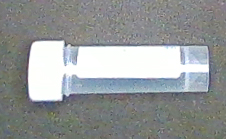
\includegraphics[width=\linewidth,keepaspectratio]{figures/fig_class_universal.png}}{\framebox[4.1cm]{\rule{0pt}{2.6cm}}}
      & Universal  & 31\,mm screw-cap     & General sample collection \\ [2pt]
    \IfFileExists{figures/fig_class_pushon.png}{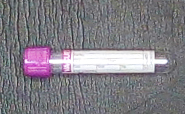
\includegraphics[width=\linewidth,keepaspectratio]{figures/fig_class_pushon.png}}{\framebox[4.1cm]{\rule{0pt}{2.6cm}}}
      & Push-on    & 13\,mm push-fit cap  & Blood collection tubes \\ [2pt]
    \IfFileExists{figures/fig_class_screwcap.png}{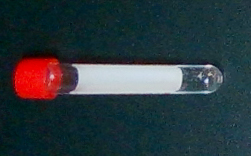
\includegraphics[width=\linewidth,keepaspectratio]{figures/fig_class_screwcap.png}}{\framebox[4.1cm]{\rule{0pt}{2.6cm}}}
      & Screwcap   & 16\,mm screw-cap     & Serum chemistry and serology sample collection \\ [2pt]
    \IfFileExists{figures/fig_class_other.png}{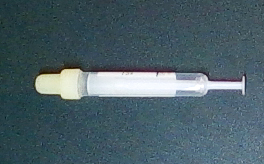
\includegraphics[width=\linewidth,keepaspectratio]{figures/fig_class_other.png}}{\framebox[4.1cm]{\rule{0pt}{2.6cm}}}
      & Other      & Non-standard         & Mixed types, manual handling \\
    \bottomrule
  \end{tabular}
  \caption{Tube classification scheme based on cap closure mechanism. Specimens shown are tubes 2 (Universal), 13 (Push-on), 27 (Screwcap), and 21 (Other); cropped RGB, no annotation.}
  \label{tab:tube_classes}
\end{table}

\subsection{Data collection and annotation}

Data was collected in two phases: an initial 17 specimens were captured first, followed by 13 further specimens to extend class coverage and balance the dataset. Each of the 30 sessions recorded 100 frames of a single tube placed individually on the matte black surface, with orientation varied across frames. Tubes were always captured one at a time, reflecting how they will enter the sorting system. A total of 3,000 RGB images were collected, each with a paired 16-bit depth map stored simultaneously, yielding 3,000 aligned RGB-D pairs. The same 70/15/15 train/validation/test split was applied to both the RGB and depth datasets.

Images were uploaded to Roboflow (version 4.0, Roboflow Inc., Des Moines, USA)~\supercite{ciaglia2022rf100} for annotation and dataset management, including export versioning and split management. Polygon segmentation masks were generated using SAM~2 (Segment Anything Model~2)~\supercite{ravi2024sam2} with click-based prompting: each tube was selected with a single click to generate a mask proposal, which was then reviewed and corrected by hand. Cap boundaries were tightened, label text regions included within the tube mask, and any background bleed trimmed. Fifteen images where SAM~2 failed to generate a mask despite manual prompting were annotated from scratch.

The annotated dataset was exported in YOLOv8 segmentation format and split into training (2\,100 images), validation (450 images), and test (450 images) subsets. To address class imbalance (Universal had the fewest instances), a rebalanced version of the dataset was also created by oversampling minority classes to equalise representation. \Cref{fig:dataset_examples} shows all 30 specimens. Humans distinguish tube classes primarily by cap size and profile: Universal caps are conspicuously wide, Push-on caps are smooth discs, Screwcap closures have a 16\,mm threaded profile, and Other encompasses non-standard designs. Cap colour provides an additional cue but is not always reliable. Screwcap and Push-on tubes are the most visually similar and can require physical handling to distinguish with certainty. \Cref{tab:class_dist} summarises the class distribution of the primary dataset.

\begin{figure}[!b]
  \centering
  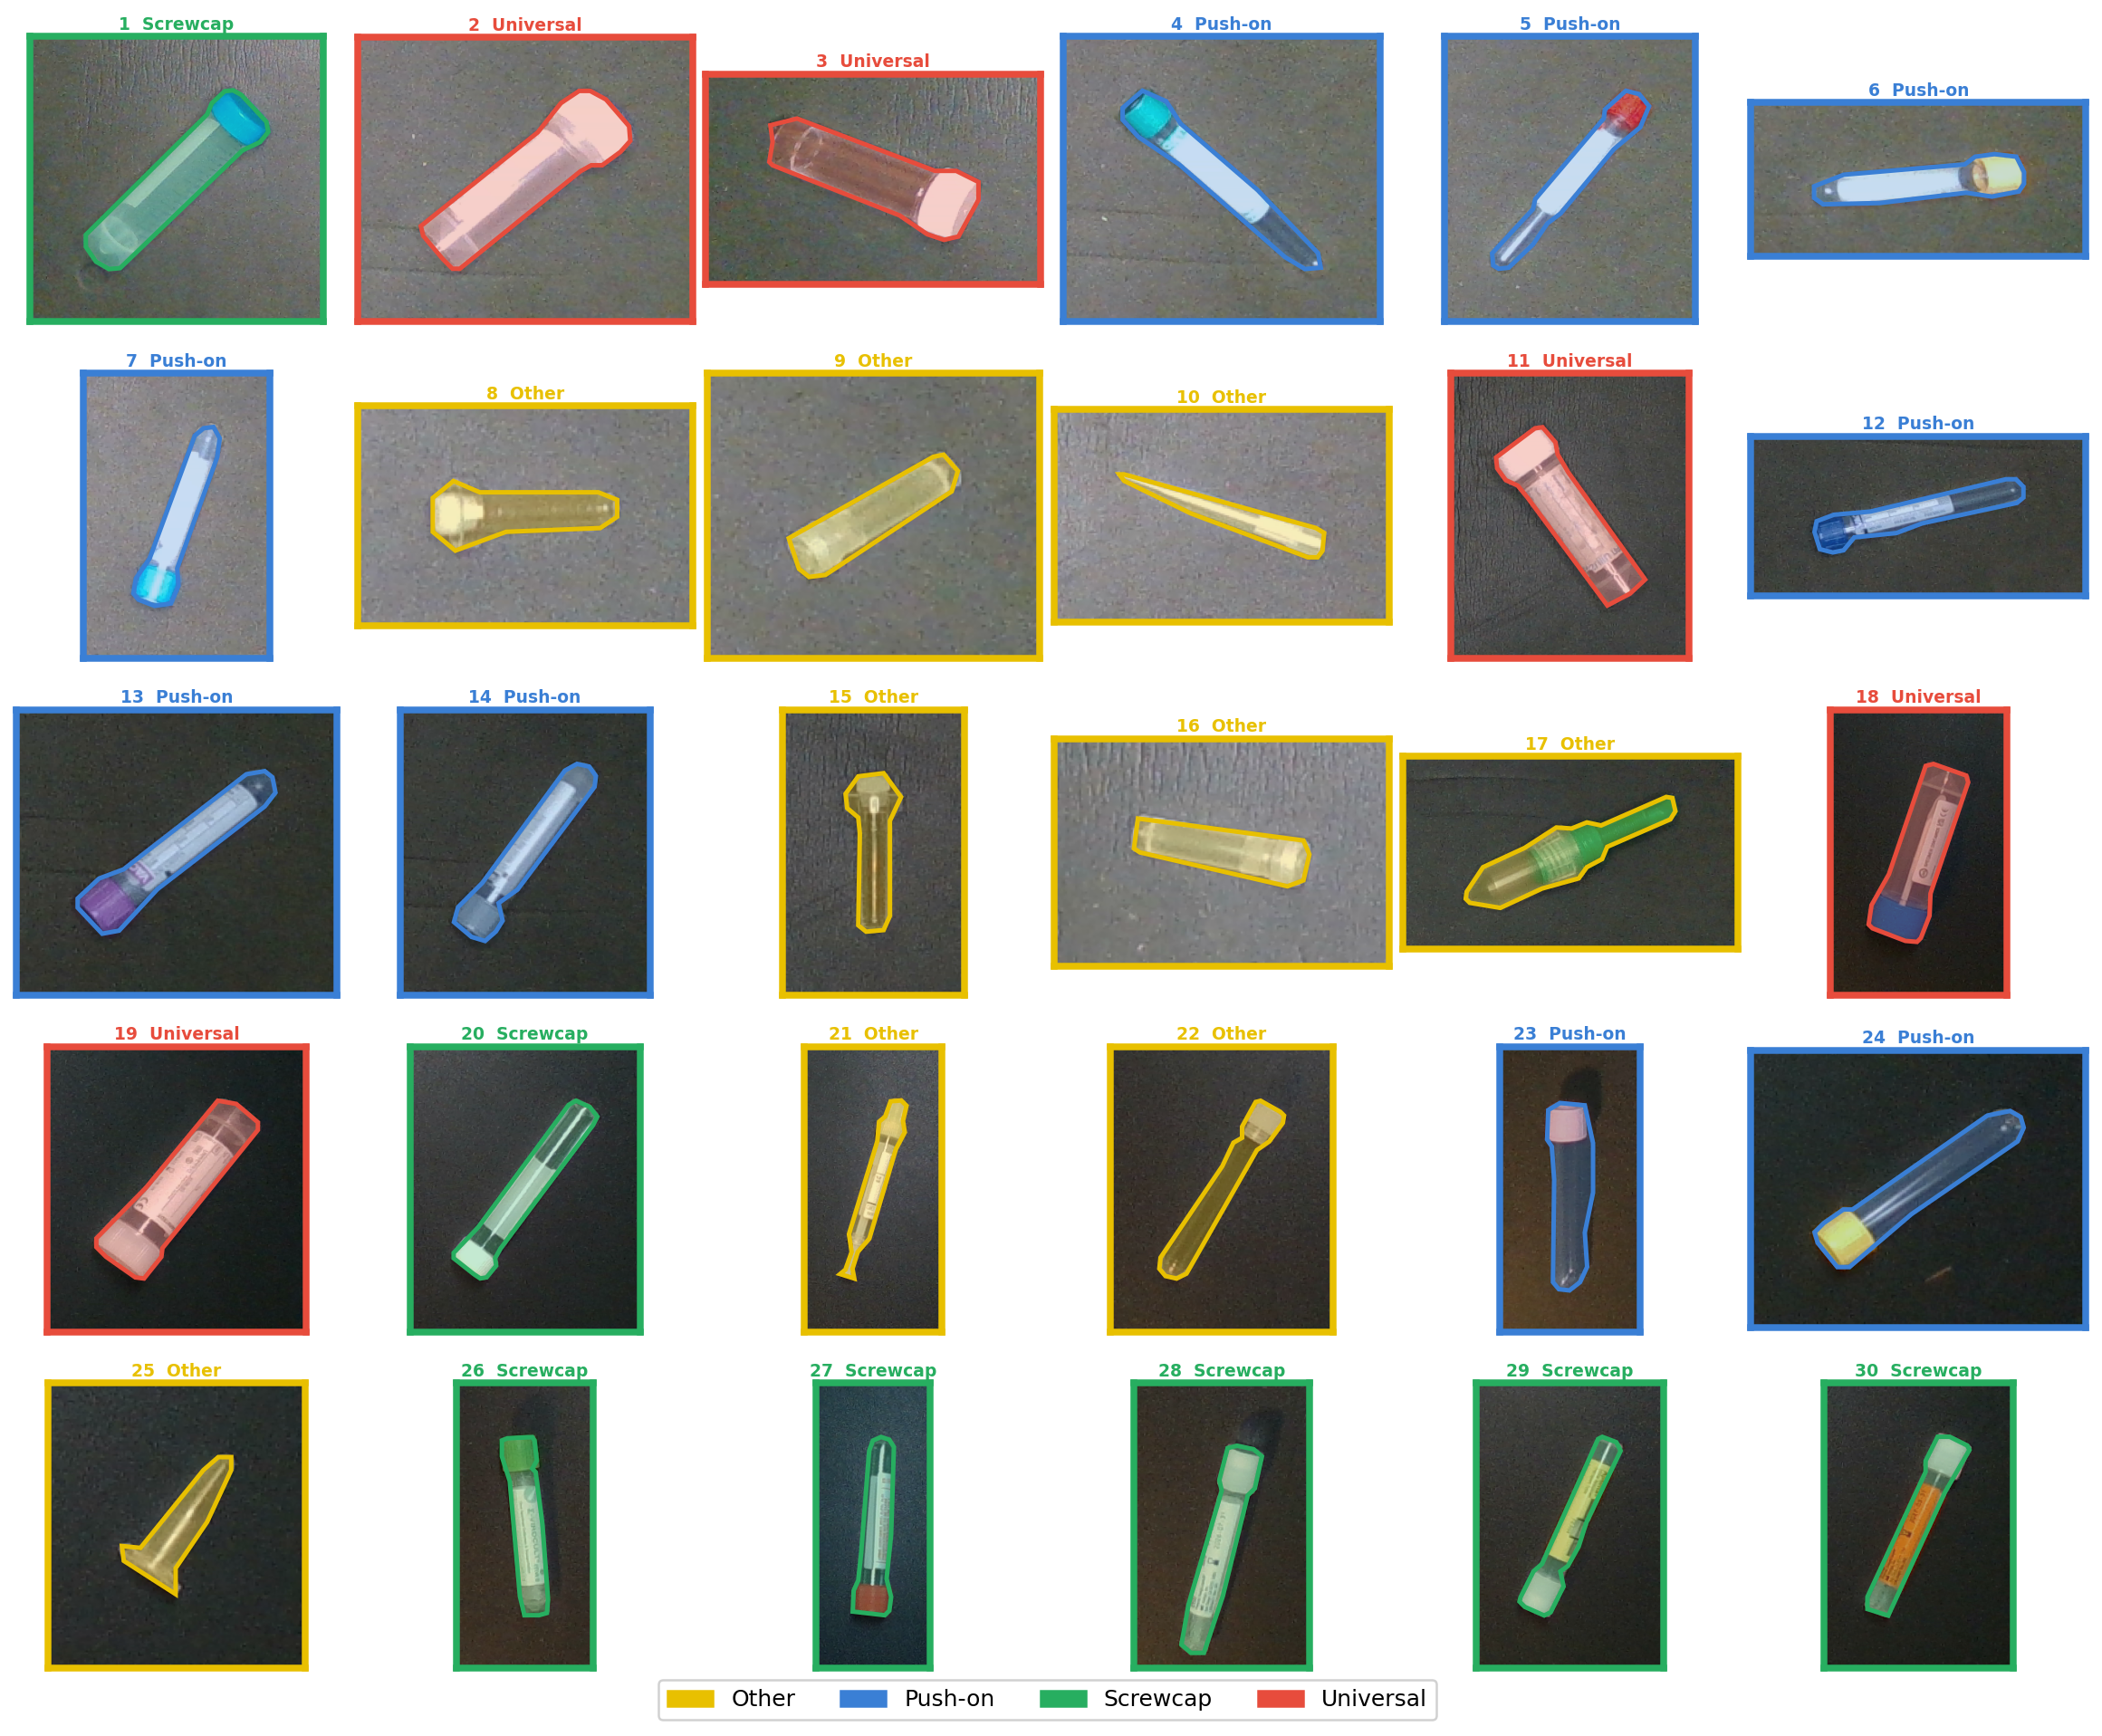
\includegraphics[width=\columnwidth]{figures/fig_dataset_examples.png}
  \caption{All 30 specimens in capture order. Segmentation polygons are colour-coded: Other (yellow), Push-on (blue), Screwcap (green), Universal (red). Coloured borders and labels indicate class.}
  \label{fig:dataset_examples}
\end{figure}

\begin{table}[!htbp]
  \centering
  \begin{tabular}{lrrrr}
    \toprule
    \textbf{Class} & \textbf{Total} & \textbf{Train} & \textbf{Valid} & \textbf{Test} \\
    \midrule
    Other      & 898  & 628  & 135 & 135 \\
    Push-on    & 895  & 626  & 134 & 135 \\
    Screwcap   & 707  & 495  & 106 & 106 \\
    Universal  & 500  & 351  &  75 &  74 \\
    \midrule
    \textbf{Total} & \textbf{3\,000} & \textbf{2\,100} & \textbf{450} & \textbf{450} \\
    \bottomrule
  \end{tabular}
  \caption{Class distribution across dataset splits. Counts reflect individual tube instances.}
  \label{tab:class_dist}
\end{table}

\subsection{Model architectures}

Five models were selected for comparison, spanning different scales and input modalities. \Cref{tab:architectures} summarises their key properties.

YOLOv8m-seg was included as a medium-scale baseline; it uses a CSP-DarkNet backbone with a Feature Pyramid Network neck~\supercite{lin2017fpn} to extract features at multiple scales. All other models are nano variants, giving a 10-fold parameter difference. The comparison assesses whether a lightweight model augmented with depth data can match a much larger RGB-only system.

\begin{table}[!htbp]
  \centering\small
  \setlength{\tabcolsep}{4pt}
  \begin{tabular}{llccp{5.0cm}p{2.8cm}}
    \toprule
    \textbf{Model} & \textbf{Input} & \textbf{Channels} & \textbf{Params} & \textbf{Key architectural features} & \textbf{Training} \\
    \midrule
    YOLOv8m-seg   & RGB   & 3 & 27.2\,M & CSPDarknet backbone, FPN neck, decoupled head & M1 Max CPU, 100\,ep \\
    YOLO11n-seg   & RGB   & 3 & 2.8\,M  & Improved feature extraction efficiency        & Cloud GPU, 100\,ep \\
    YOLO26n-seg   & RGB   & 3 & 2.7\,M  & NMS-free end-to-end, anchor-free              & Cloud GPU, 100\,ep \\
    YOLO11n-RGBD  & RGB-D  & 4 & 2.8\,M  & Modified first conv, 4-channel RGB-D input    & M1 Max CPU, 100\,ep \\
    YOLO26n-depth & Depth & 1 & 2.7\,M  & Depth channel normalised to 8-bit; replicated to 3 for network input & Cloud GPU, 100\,ep \\
    \bottomrule
  \end{tabular}
  \caption{Model architectures compared in this study.}
  \label{tab:architectures}
\end{table}

\subsection{Training configuration}

YOLOv8m-seg was trained locally on the M1~Max CPU using PyTorch~2.12.0~\supercite{paszke2019pytorch} with the Ultralytics framework (v8.4.56). No dedicated graphics processing unit was available. Apple Metal Performance Shaders (MPS) support was verified, but training defaulted to CPU for stability due to occasional numerical differences on the MPS backend. Training ran for 100~epochs, taking over 50 hours, with batch size~8, image size~640, AdamW optimiser (lr$_0$\,=\,0.01, weight decay\,=\,0.0005), and early stopping patience of 20 epochs. The learning rate followed a cosine annealing schedule (0.01$\to$0.0001).

Data augmentation followed the mosaic strategy~\supercite{bochkovskiy2020yolov4,shorten2019augmentation}, which combines four training images into a single composite to increase object diversity per batch. Additional augmentations included: horizontal and vertical flip (probability~0.5 each), HSV hue jitter\,=\,0.015, saturation jitter\,=\,0.7, value jitter\,=\,0.4, rotation up to 180\textdegree{}, scale\,=\,0.5, perspective warp\,=\,0.0005, and random erasing\,=\,0.4 to simulate partial occlusion. The aggressive rotation range was justified by the controlled overhead capture setup: tubes can appear at any angle relative to the camera and have no inherent ``upright'' orientation.

Three models were trained on Roboflow's cloud GPU infrastructure. YOLO11n-seg and YOLO26n-seg used the RGB dataset with default augmentation presets. YOLO26n-depth used the depth-only dataset, with each single-channel image replicated to three channels to match the network's expected input format.

For the RGB-D experiment, paired depth maps were aligned to RGB frames using the RealSense SDK and appended as a fourth channel. The 16-bit depth values were normalised to the 0--255 range based on the calibrated scene depth range, then appended to the 8-bit RGB channels. The YOLO11n architecture was modified at the first convolutional layer to accept 4-channel input. YOLO11n-RGBD was trained locally on the M1~Max CPU for 100~epochs using the same augmentation settings as the RGB models.

A YOLO26n model was additionally trained on the class-balanced dataset to evaluate whether equalising class representation improves minority-class performance. The balanced dataset was constructed by oversampling images containing minority classes (Screwcap, Universal) to achieve approximately equal instance counts across all four classes.

\subsection{Evaluation protocol}

All RGB models were evaluated on the 450-image held-out test split using standard COCO metrics~\supercite{lin2014coco,padilla2020survey}: bounding-box mAP at IoU\,=\,0.50 (mAP\textsubscript{50}) and averaged over IoU thresholds \mbox{0.50--0.95} in steps of 0.05 (mAP\textsubscript{50--95}). Mask mAP was computed for all models by measuring the IoU between predicted and ground-truth segmentation polygons at the same threshold range. Precision and recall were computed at IoU\,=\,0.50 for both box and mask predictions. Inference speed was measured as end-to-end latency per image (including pre-processing, forward pass, and post-processing) on the M1~Max CPU, averaged over the full test set. All evaluations used the Ultralytics validation pipeline with batch size~8 and image size~640. To quantify test-set sampling uncertainty, 500-iteration image-level bootstrap resampling was applied to model predictions using the COCO evaluation API~\supercite{efron1994bootstrap}; the resulting bootstrap standard deviation of mask~mAP\textsubscript{50--95} was 0.008, giving a 95\% margin of $\pm$0.015 per model and a two-model comparison threshold of $\approx$0.022.

\begin{figure}[!htbp]
  \centering
  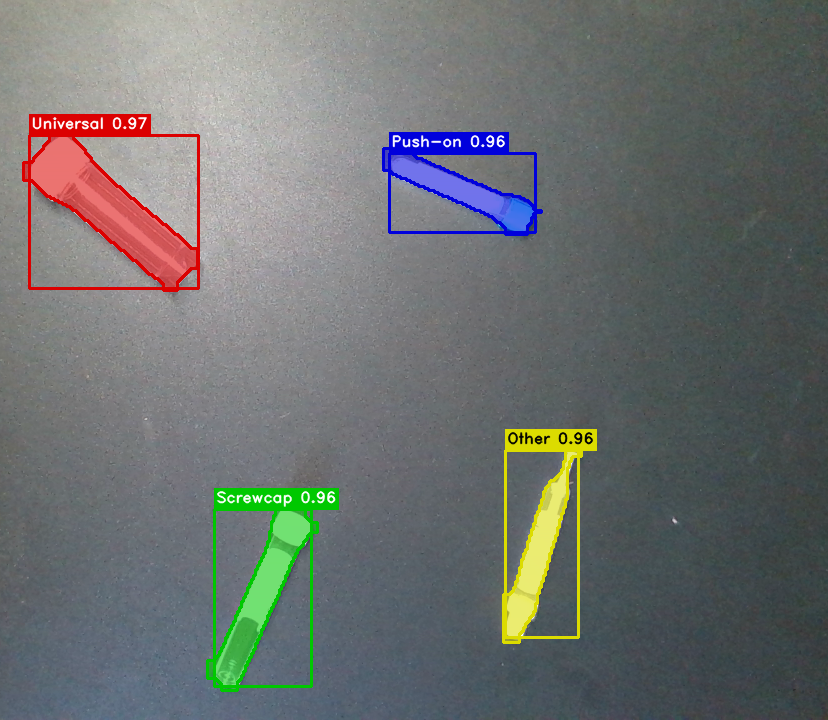
\includegraphics[width=\columnwidth]{figures/fig_all_classes.png}
  \caption{All four tube classes detected simultaneously with YOLO26n-seg. Universal (red, 0.97), Push-on (blue, 0.96), Screwcap (green, 0.96), and Other (yellow, 0.96). Masks show pixel-level segmentation boundaries.}
  \label{fig:all_classes}
\end{figure}

%%====================================================================
\section{Results}
%%====================================================================

\subsection{Model comparison}

\Cref{tab:model_comparison} presents the test-set performance of all five models. YOLOv8m-seg achieved the highest mask~mAP\textsubscript{50--95} of 0.905 among RGB-only models with its 27.2\,M~parameters. Among lightweight models, YOLO26n-seg and YOLO11n-seg reached identical mask~mAP\textsubscript{50--95} of 0.820; YOLO26n-seg is 1.4\,ms slower at 23.1\,ms/frame. \Cref{fig:all_classes} shows a representative live inference result with all four tube classes correctly detected and segmented. Confidence scores across all four classes ranged from 0.96 to 0.97, with no confusion between classes.

\begin{table}[!htbp]
  \centering
  \begin{tabular}{llccccc}
    \toprule
    \textbf{Model} & \textbf{Input} & \textbf{Params} & \textbf{Ep.} & \textbf{Box mAP\textsubscript{50--95}} & \textbf{Mask mAP\textsubscript{50--95}} & \textbf{ms/img} \\
    \midrule
    YOLO11n-RGBD  & RGB-D  & 2.8\,M  & 100 & 0.988 & 0.929 & 22.4 \\
    YOLOv8m-seg   & RGB   & 27.2\,M & 100 & 0.968 & 0.905 & 108.5 \\
    YOLO26n-seg   & RGB   & 2.7\,M  & 100 & 0.951 & 0.820 & 23.1 \\
    YOLO11n-seg   & RGB   & 2.8\,M  & 100 & 0.949 & 0.820 & 21.7 \\
    YOLO26n-depth & Depth & 2.7\,M  & 100 & 0.919 & 0.804 & 22.8 \\
    \bottomrule
  \end{tabular}
  \caption{Model comparison at 640$\times$640. Inference on M1~Max CPU. Ep.\ = training epochs. Sorted by mask~mAP\textsubscript{50--95}.}
  \label{tab:model_comparison}
\end{table}

Two observations stand out from \Cref{fig:model_comparison}: first, the gap between box and mask accuracy is consistent across all models, confirming polygon regression is harder than bounding-box detection regardless of architecture; second, the RGB-D model achieves the highest values on both metrics despite having the same parameter count as the other nano models, making it the clear choice when a depth camera is available.

\begin{figure}[!b]
  \centering
  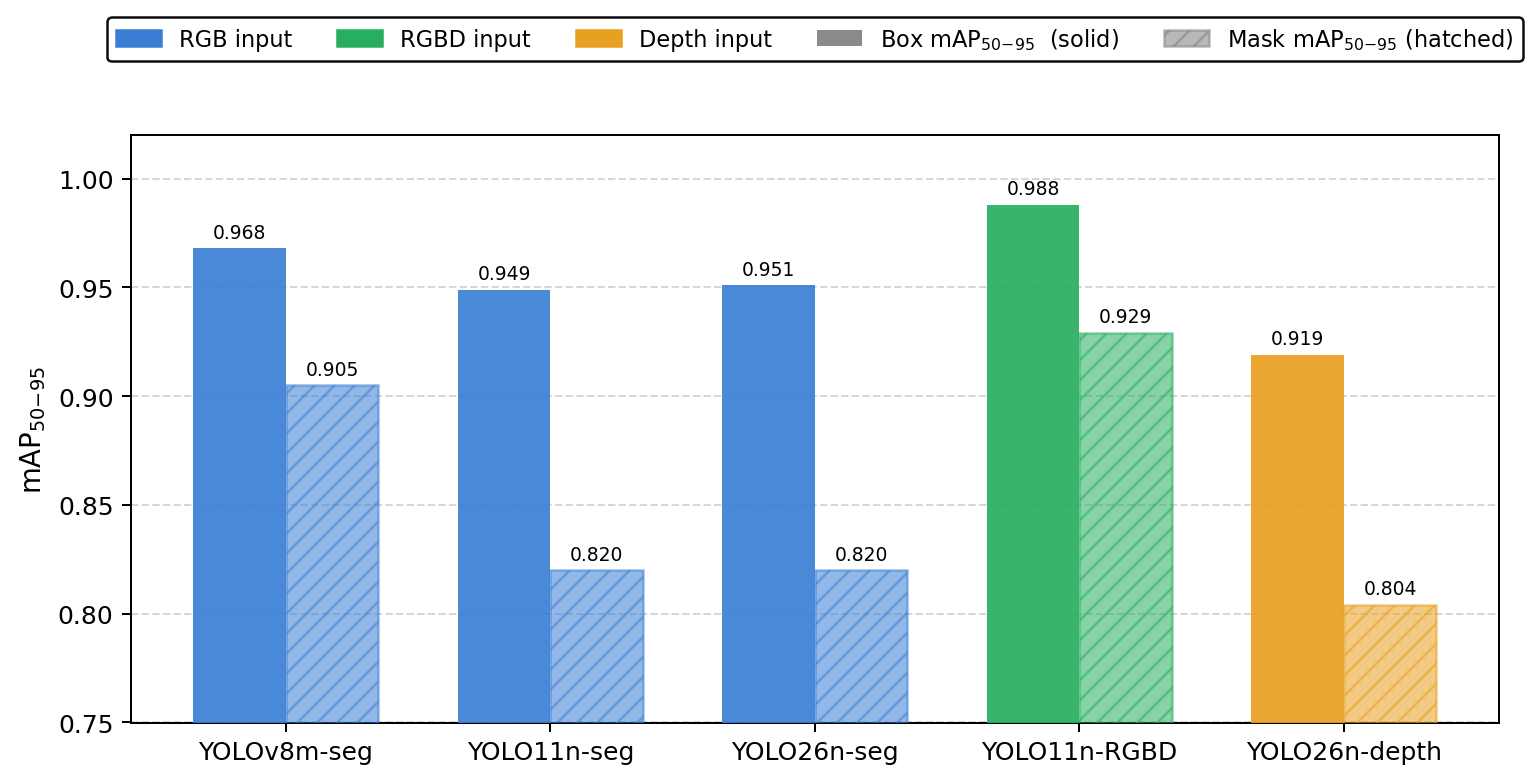
\includegraphics[width=\columnwidth]{figures/fig_model_comparison.png}
  \caption{Grouped bar chart comparing box~mAP\textsubscript{50--95} (solid bars) and mask~mAP\textsubscript{50--95} (hatched bars) for all five models. Input modality: blue for RGB, green for RGB-D, orange for depth-only. YOLO11n-RGBD achieves the highest mask score despite using only 2.8\,M~parameters.}
  \label{fig:model_comparison}
\end{figure}

Bootstrap resampling (500 iterations over the 450-image test set, 95\% margin $\pm$0.015) confirms that the RGB-D advantage of 0.024 over YOLOv8m-seg marginally exceeds the two-model significance threshold of 0.022, while the 0.109 advantage over nano RGB models is unambiguous, and the zero difference between YOLO26n-seg and YOLO11n-seg confirms these models are statistically indistinguishable.

\subsection{Depth-channel experiments}

The RGB-D four-channel model (YOLO11n-RGBD) achieved the highest mask~mAP\textsubscript{50--95} of 0.929 and box~mAP\textsubscript{50--95} of 0.988 across all models. This shows that adding the depth channel to a lightweight nano model can exceed the accuracy of a much larger RGB-only model (YOLOv8m-seg, 27.2\,M~parameters) while running at nearly the same speed as the nano baseline. The RGB-D model was trained and evaluated on the full 3,000-image paired RGB-D dataset with the same 70/15/15 train/validation/test split used for the RGB models, ensuring the performance advantage reflects genuine cross-set generalisation. The improvement is most pronounced for geometrically similar classes: Screwcap and Push-on tubes can feature caps in similar colour shades, but the 16\,mm Screwcap has a wider threaded cap than the 13\,mm Push-on, a geometric difference directly encoded in the depth channel.

The depth-only single-channel model (YOLO26n-depth) achieved 0.804 mask~mAP\textsubscript{50--95}, showing that geometric shape information alone---without any colour---provides enough information for tube classification. This result was surprising given that cap colour is the most visually obvious distinguishing feature to human observers. The model appears to have learned class-discriminative shape features: Push-on caps have a characteristic flat disc profile at one end, Universal tubes are wider with a prominent threaded collar, Screwcap tubes have a narrower threaded profile, and Other tubes have irregular or elongated closure geometries. These shape differences, while subtle to the human eye in 2D images, produce distinct depth signatures when viewed from above.

The practical value of depth extends beyond accuracy: in clinical environments, tubes may become discoloured, label adhesive may obscure cap colours, or overhead lighting may produce specular reflections; a depth-based model is inherently immune to these visible-light failure modes. This makes depth well-suited to hospital waste-sorting stations where lighting is routinely inconsistent.

\subsection{Per-class analysis}

\Cref{tab:perclass} shows the per-class test results for YOLOv8m-seg. Box detection was near-perfect across all classes (mAP\textsubscript{50}\,$\geq$\,0.954). The largest mask-quality gap appeared for the Other class, where mAP\textsubscript{50--95} dropped to 0.748, partly because its irregular profiles were occasionally assigned background confidence by the model. Correctly classifying Other is clinically important: these tubes require manual intervention, and routing them to the wrong stream would contaminate single-polymer recovery batches. Universal tubes, with their symmetrical cylindrical geometry, achieved the highest mask~mAP\textsubscript{50--95} of 0.887. Training on the class-balanced dataset improved Screwcap and Universal detection consistency, confirming that the imbalance between classes affected minority-class performance. \Cref{fig:confusion} shows the normalised confusion matrix for YOLOv8m-seg on the test split.

\begin{table}[!htbp]
  \centering
  \begin{tabular}{lcccc}
    \toprule
    \textbf{Class} & \textbf{Box mAP\textsubscript{50}} & \textbf{Box mAP\textsubscript{50--95}} & \textbf{Mask mAP\textsubscript{50}} & \textbf{Mask mAP\textsubscript{50--95}} \\
    \midrule
    All        & 0.985 & 0.968 & 0.985 & 0.806 \\
    Other      & 0.995 & 0.957 & 0.995 & 0.748 \\
    Push-on    & 0.995 & 0.978 & 0.995 & 0.791 \\
    Screwcap   & 0.954 & 0.945 & 0.954 & 0.798 \\
    Universal  & 0.995 & 0.993 & 0.995 & 0.887 \\
    \bottomrule
  \end{tabular}
  \caption{Per-class results for YOLOv8m-seg (best checkpoint, epoch~85) on the 450-image test split.}
  \label{tab:perclass}
\end{table}

\begin{figure}[!htbp]
  \centering
  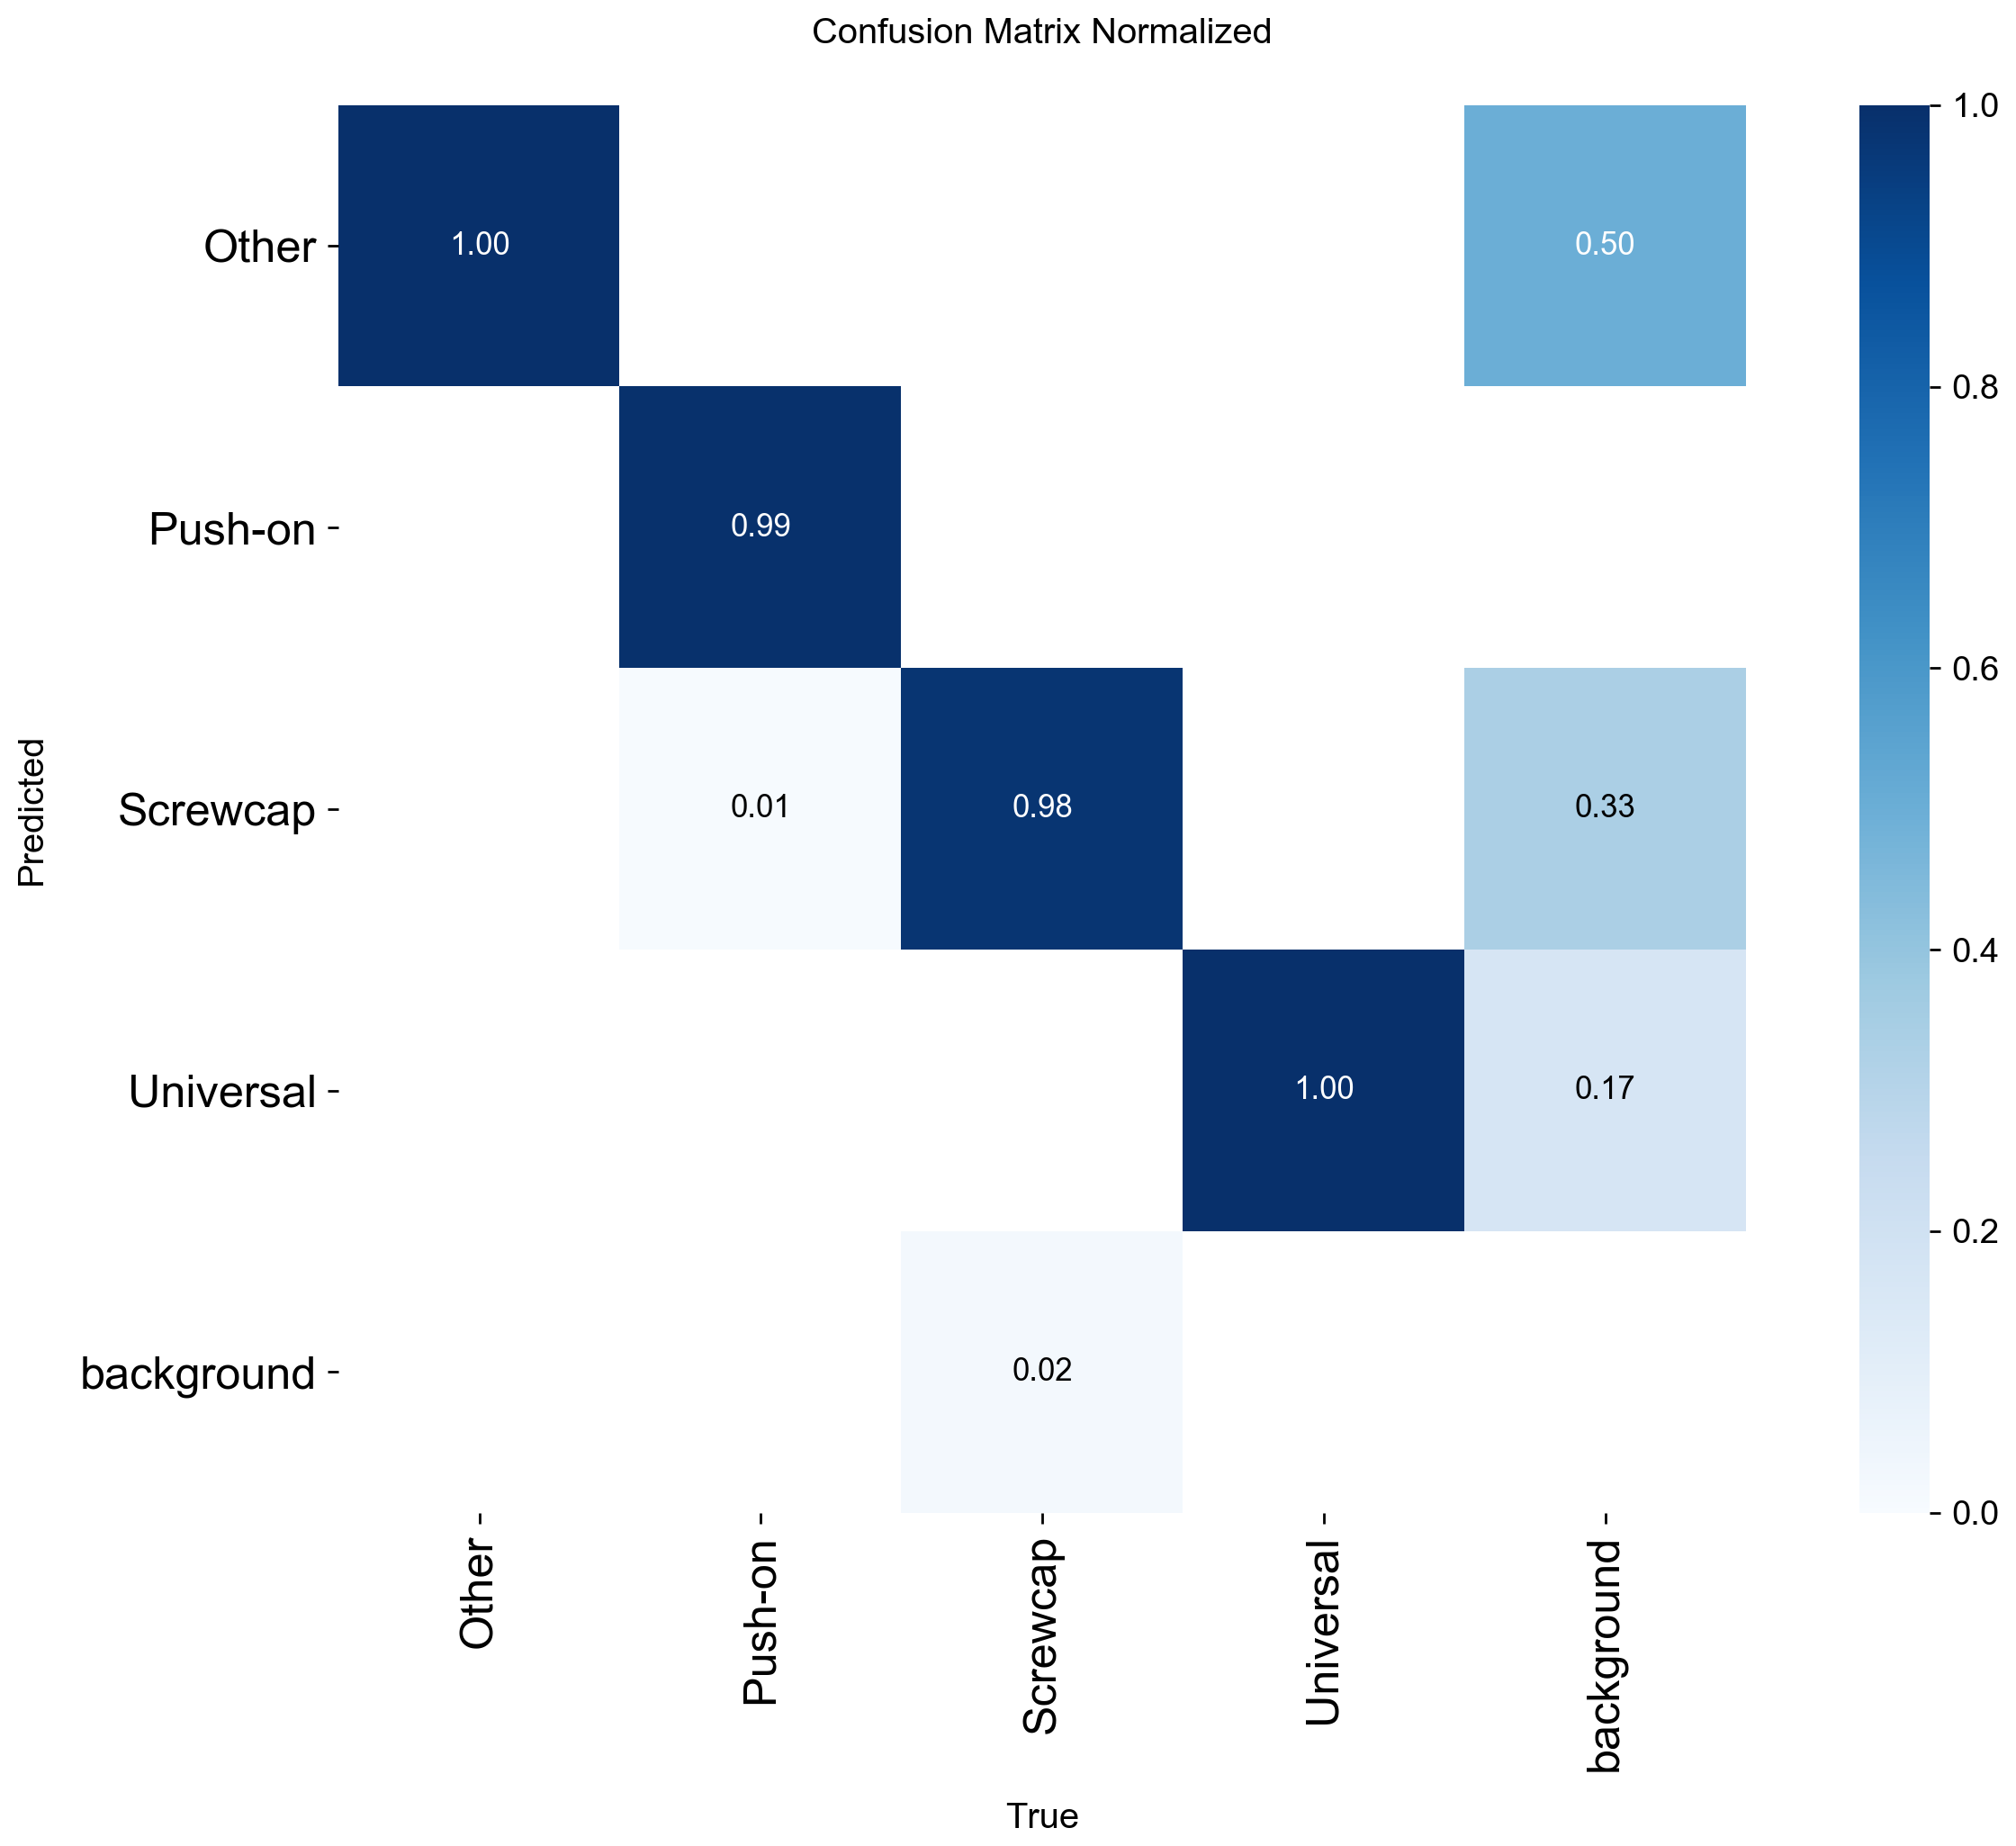
\includegraphics[width=\columnwidth]{figures/fig_confusion_matrix.png}
  \caption{Normalised confusion matrix for YOLOv8m-seg on the 450-image test split. Diagonal values close to 1.0 indicate high classification accuracy. The main source of confusion is between Screwcap and Push-on classes, consistent with their visual similarity.}
  \label{fig:confusion}
\end{figure}

\subsection{Training dynamics}

The YOLOv8m-seg training run reached peak validation mask~mAP\textsubscript{50--95} of 0.911 at epoch~85, after which performance plateaued. Box losses converged smoothly from epoch~20, while mask losses showed higher variance; no overfitting was observed. \Cref{fig:training} shows the metric curves over 100~epochs. The persistent gap between box~mAP\textsubscript{50--95} (0.968) and mask~mAP\textsubscript{50--95} (0.905) throughout training suggests that the primary ceiling on mask quality is not model capacity.

\begin{figure}[!htbp]
  \centering
  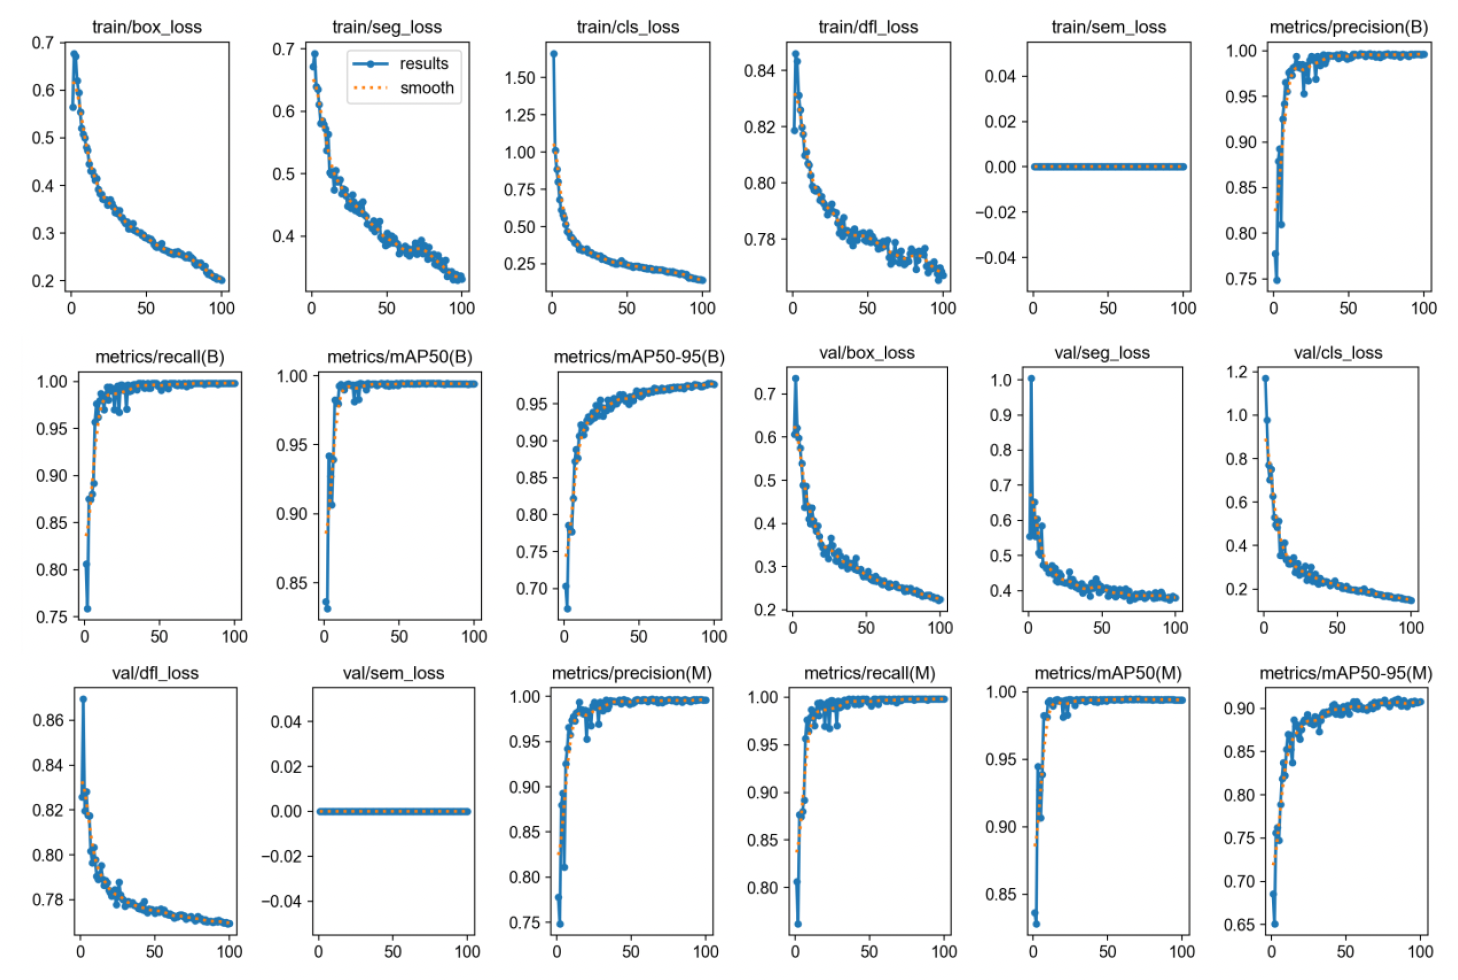
\includegraphics[width=\columnwidth]{figures/fig_training_curves.png}
  \caption{YOLOv8m-seg training and validation metrics over 100~epochs. Losses converge rapidly in the first 20 epochs and plateau from epoch 70; validation curves track training closely, confirming no overfitting. The persistent gap between box and mask mAP throughout training reflects the difficulty of polygon regression. Peak validation mask~mAP\textsubscript{50--95} of 0.911 was reached at epoch 85.}
  \label{fig:training}
\end{figure}

\subsection{Real-time inference}

A live inference pipeline was implemented using YOLO26n-seg, capturing aligned RGB and depth frames at 30\,fps and rendering a four-panel display (\Cref{fig:pipeline}): raw RGB stream, RGB with colour-coded segmentation overlays at 50\% opacity, depth heatmap, and depth with masks projected. Models can be switched at runtime; snapshot capture and continuous recording at 2\,fps are supported. Nano models reach 30--45\,fps; YOLOv8m-seg runs at approximately 9\,fps on the M1~Max CPU.

\begin{figure}[!htbp]
  \centering
  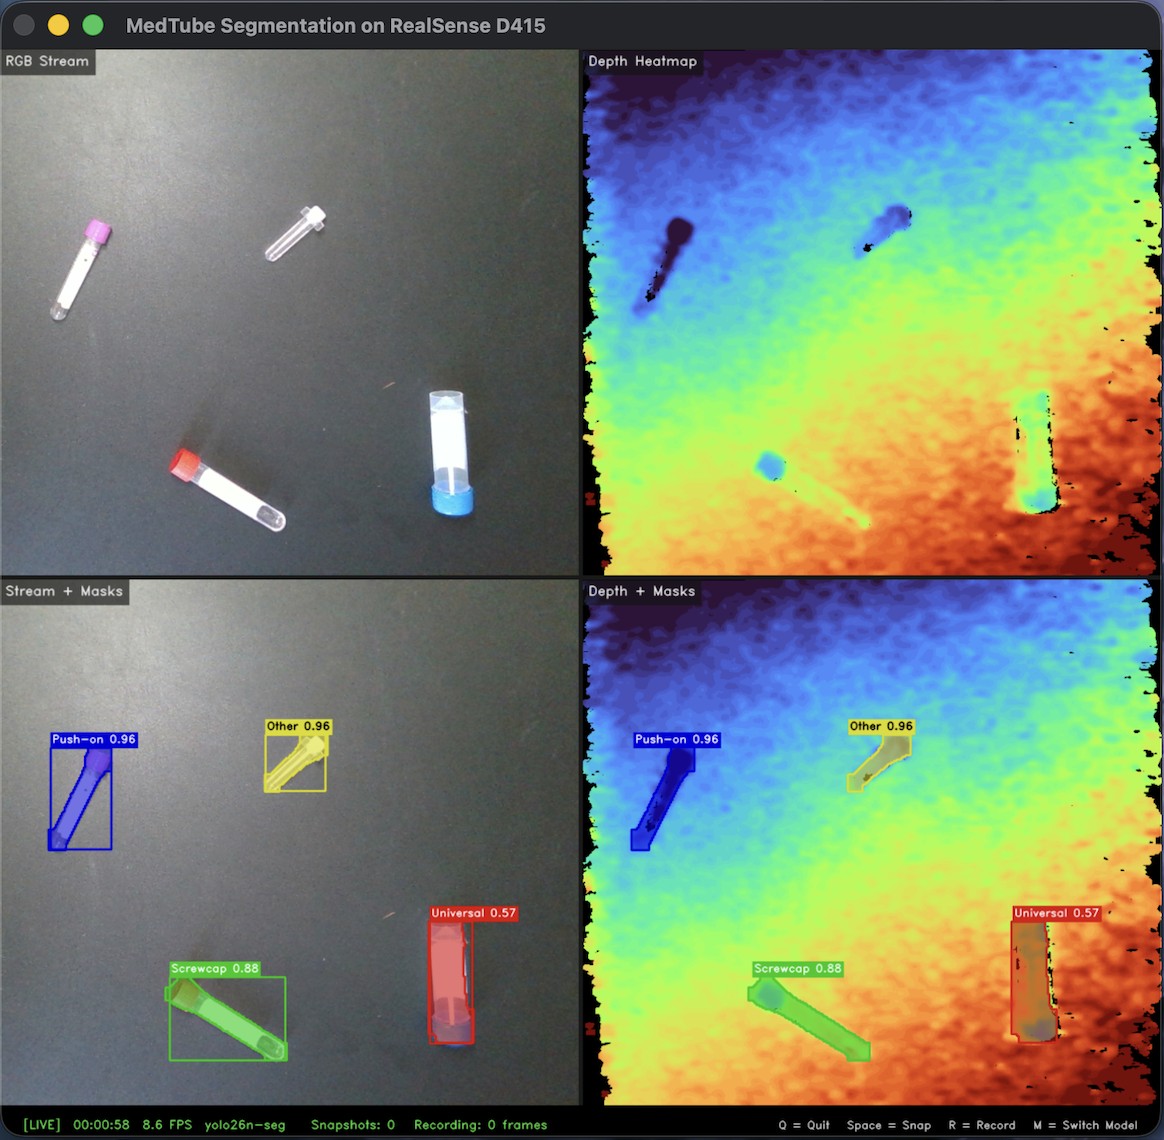
\includegraphics[width=\columnwidth]{figures/fig_pipeline_grid.png}
  \caption{Live inference pipeline showing the 2$\times$2 display grid as seen by the operator. Top-left: raw RGB stream. Top-right: RGB with segmentation masks. Bottom-left: depth heatmap (TURBO colourmap). Bottom-right: depth with masks overlaid. The HUD bar shows current model, recording state, FPS, and session statistics.}
  \label{fig:pipeline}
\end{figure}

Nano models reach 30--45\,fps; YOLOv8m-seg runs at approximately 9\,fps on the M1~Max CPU.

%%====================================================================
\section{Discussion}
%%====================================================================

\subsection{Model scale and accuracy}

The results show a clear trade-off between model size and segmentation accuracy. The medium-scale YOLOv8m-seg (27.2\,M~parameters) achieved the highest RGB mask~mAP\textsubscript{50--95} of 0.905, while the nano-scale models (YOLO11n, YOLO26n, both $\sim$2.7\,M~parameters) reached 0.820---a 9.4\% relative drop---while being 4.7$\times$ faster. For real-time deployment where latency is critical, this trade-off is acceptable: a 21.7\,ms inference time corresponds to 46\,fps, well above the 30\,fps camera rate. The speed difference is particularly apparent in the live stream: YOLOv8m-seg runs at approximately 9\,fps with noticeable lag when tubes are moved, while the nano models track movement smoothly.

Importantly, adding a depth channel to the nano architecture (YOLO11n-RGBD) recovered most of this accuracy gap at 0.929 mask~mAP\textsubscript{50--95} without increasing inference time, confirming that depth fusion is more practical than model scaling for this application.

\subsection{Class-level performance and annotation quality}

Screwcap exhibited the lowest detection mAP\textsubscript{50} (0.954 versus 0.995 for other classes). This is partly explained by the lower instance count (707 versus 895 for Push-on) and the visual similarity between Screwcap and Push-on tubes: although the 16\,mm Screwcap has a wider threaded cap than the 13\,mm Push-on, the difference can be subtle from an overhead camera angle and both cap types appear in similar colour ranges. \Cref{fig:screwcap_comparison} shows this in practice: the nano model (YOLO26n-seg) misclassifies one Screwcap tube as Push-on with low confidence (0.57), while the larger YOLOv8m-seg correctly identifies all three tubes with high confidence (0.91--0.97).

The gap between mask~mAP\textsubscript{50} and mask~mAP\textsubscript{50--95} (0.985 versus 0.806 overall) has two concurrent causes: annotation polygon coarseness and the architectural prototype-mask constraint~\supercite{bolya2019yolact}. YOLO-seg masks are linear combinations of 32 basis prototypes; this bounds mask precision for elongated cap profiles regardless of annotation quality, meaning finer annotation alone cannot close the full gap. The confusion matrix (\Cref{fig:confusion}) confirms that dominant errors are classification-level (Screwcap\,$\leftrightarrow$\,Push-on) rather than localisation failures~\supercite{hoiem2012diagnosing}.

\begin{figure}[!htbp]
  \centering
  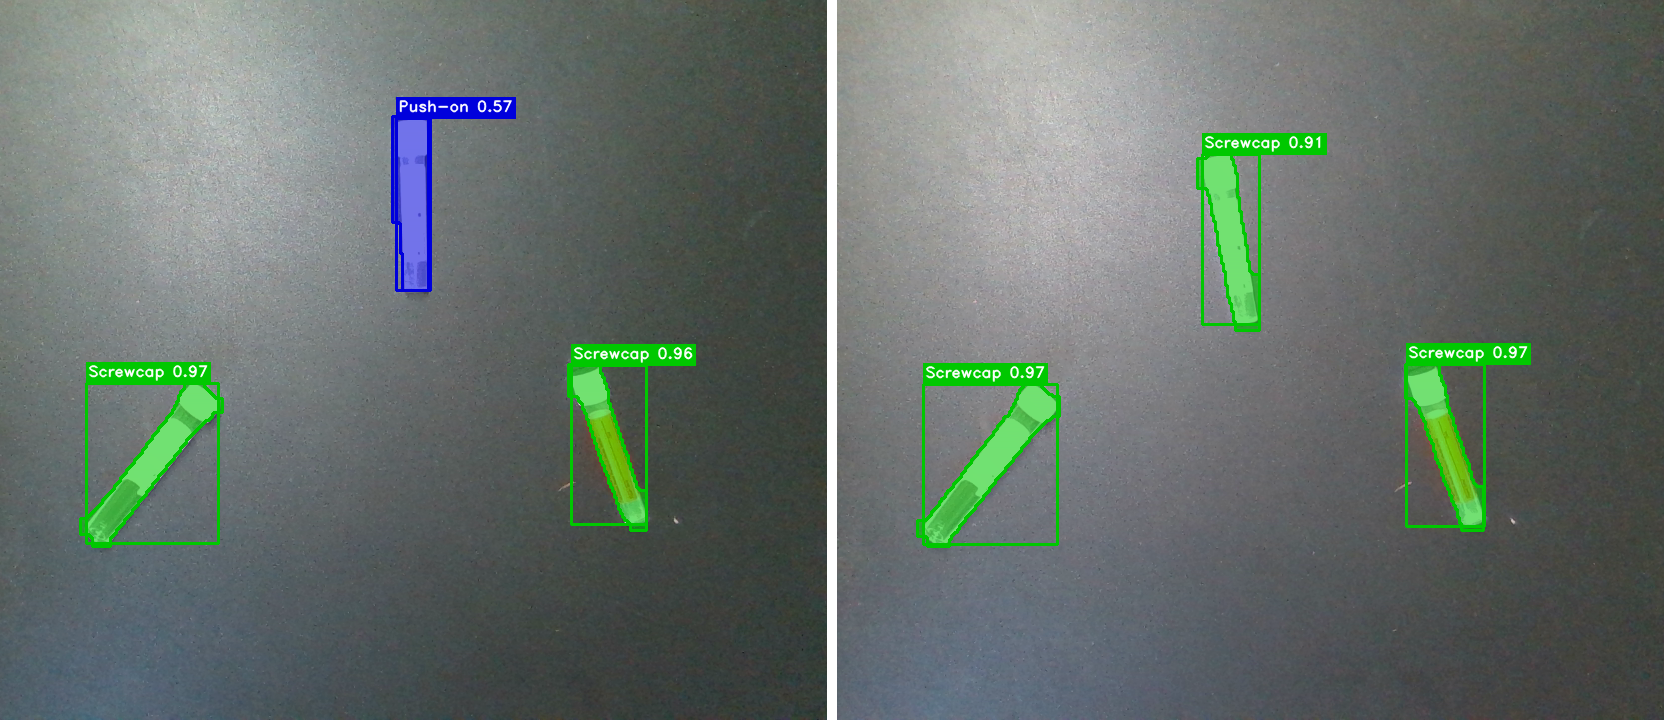
\includegraphics[width=\columnwidth]{figures/fig_screwcap_comparison.png}
  \caption{Screwcap detection comparison. Left: YOLO26n-seg misclassifies one tube as Push-on (0.57). Right: YOLOv8m-seg correctly identifies all three as Screwcap (0.91--0.97), demonstrating the accuracy benefit of larger architectures.}
  \label{fig:screwcap_comparison}
\end{figure}

Training on the class-balanced dataset confirmed that the imbalance affected results: minority classes (Screwcap, Universal) showed more consistent detection when class representation was equalised during training.

\begin{figure}[!b]
  \centering
  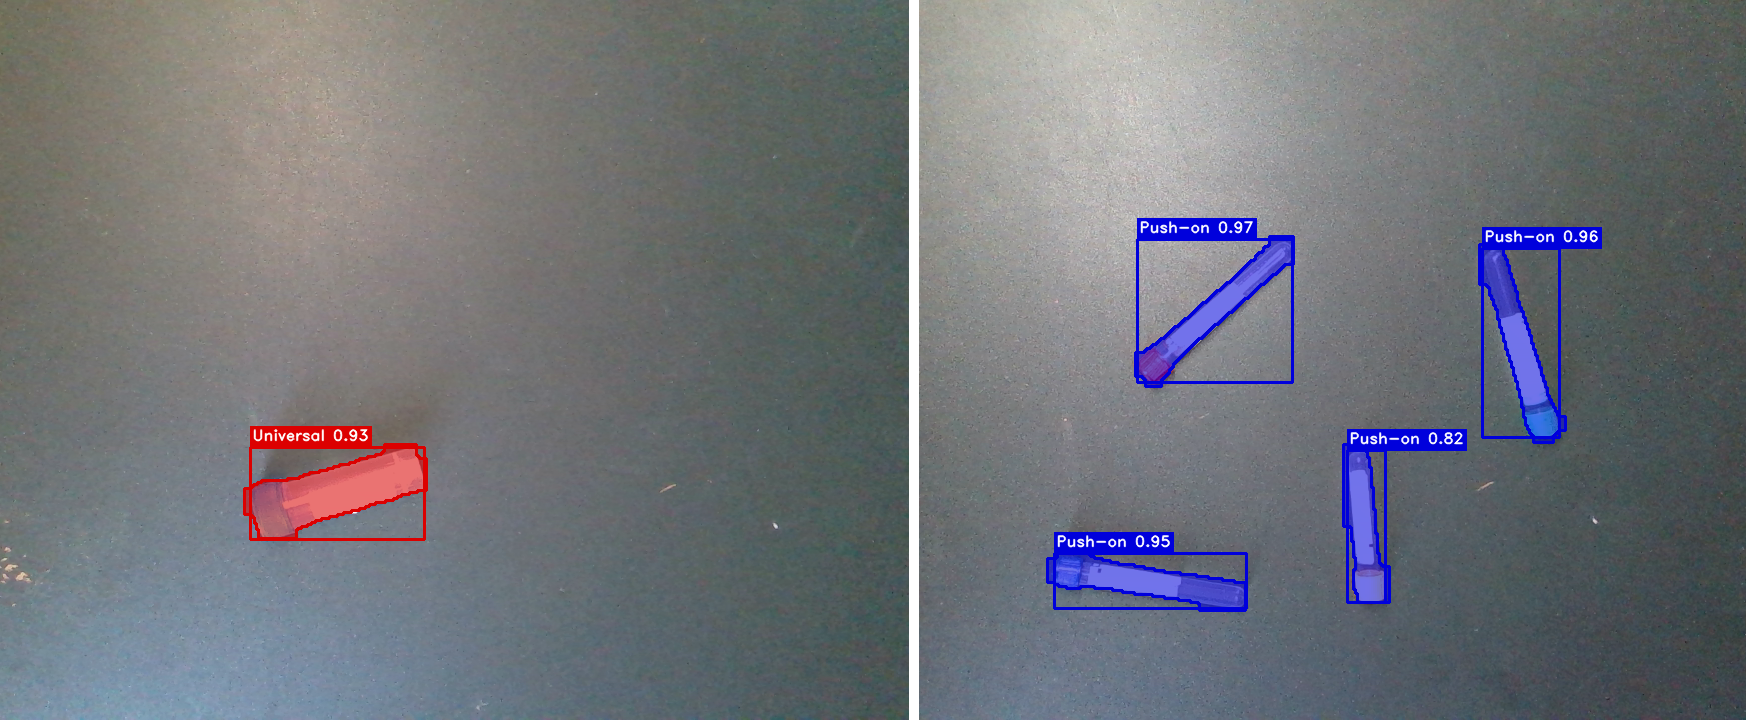
\includegraphics[width=\columnwidth]{figures/fig_inference_pair.png}
  \caption{Live inference examples. Left: single Universal tube detected at 0.93 confidence. Right: four Push-on tubes detected simultaneously with confidences of 0.82--0.97, demonstrating correct multi-instance segmentation.}
  \label{fig:inference_pair}
\end{figure}

\subsection{Depth integration}

The RGB-D experiments show that depth fusion improves segmentation quality: YOLO11n-RGBD's mask~mAP\textsubscript{50--95} of 0.929 exceeds even the much larger YOLOv8m-seg (0.905). The depth channel provides shape information where colour is less reliable---Screwcap and Universal tubes differ in cap height, a feature directly captured in the depth map.

The depth-only model's strong performance (0.804 mask~mAP\textsubscript{50--95}) confirms that tube geometry alone carries enough class information for accurate classification. Under varying clinical lighting, specular highlights and colour shifts can confuse RGB-only classifiers; a depth-based model is inherently robust, since the infrared stereo measurement is unaffected by visible-light conditions. This makes depth particularly well-suited to hospital waste-sorting stations, where lighting is routinely inconsistent. \Cref{fig:depth} shows the depth heatmap captured by the RealSense D415.

\begin{figure}[!b]
  \centering
  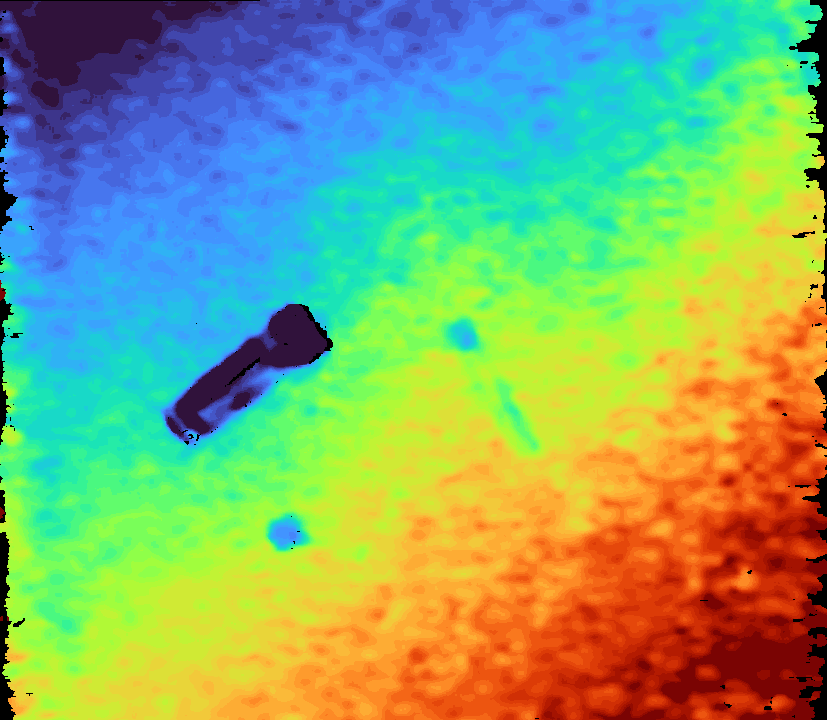
\includegraphics[width=\columnwidth]{figures/fig_depth_heatmap.png}
  \caption{Depth heatmap from the Intel RealSense D415 (TURBO colourmap, 2nd--98th percentile range). Warmer colours indicate greater distance from the camera. The flat matte surface provides a uniform depth baseline against which tube geometry is clearly distinguishable.}
  \label{fig:depth}
\end{figure}

A depth-only deployment requires no colour camera and is robust to tube staining, wetting, and variable lighting. The 7.5 percentage point gap confirms colour adds meaningful information under controlled conditions, but 0.804 is sufficient for a functional controlled-environment sorter. The 0.024 RGB-D improvement over YOLOv8m-seg (marginally significant under bootstrap analysis) is consistent with late-fusion RGB-D findings~\supercite{eitel2015rgbd} that depth fusion is more hardware-efficient than model scaling.

\subsection{Limitations}

Several limitations should be noted. First, no dedicated GPU was available; training defaulted to the Apple M1~Max CPU, taking over 50 hours per model and precluding systematic hyperparameter search. GPU access would have enabled larger model variants and faster experimental iteration. Second, data were captured with tubes stationary on a flat surface. The conveyor belt hardware was still in production at the time of writing, so the system has not been tested under dynamic conditions such as motion blur and tube tumbling. An intermediate test on a tabletop conveyor at progressively higher speeds would establish how performance degrades before the production system is ready.

Third, all training and evaluation specimens are unused and uncontaminated. Testing with post-use tubes containing blood residue or biological contamination would pose an infection risk that cannot be safely managed in a university laboratory---the same contamination hazard that makes manual sorting unsafe in the first place. Evaluation on real post-use specimens, under appropriate biosafety protocols, must be completed before clinical deployment. Fourth, the dataset covers only one manufacturer (Greiner Bio-One VACUETTE). Tubes from other common suppliers such as BD Vacutainer and Sarstedt Monovette differ in label design, cap colour, and surface texture in ways that may cause misclassification in a mixed-brand facility. Cross-manufacturer evaluation is required before deployment across multiple hospital sites.

The system does, however, produce zero false positives on an empty scene, indicating that the models have learned meaningful tube features rather than simply detecting any object in the field of view. This is an important validation for deployment scenarios where the camera may observe the sorting surface between tube arrivals.

\subsection{Impact statement}

Accurate tube classification directly enables circular economy recovery: each correctly classified tube enters the appropriate disassembly, decontamination, and reuse stream rather than incineration. Polypropylene tubes are 70--80\% recoverable when properly segregated by type~\supercite{lee2004medical}, yet most are currently incinerated alongside hazardous waste because manual sorting at scale is unsafe for workers. Incinerating one tonne of clinical waste produces approximately 0.5\,tonnes CO\textsubscript{2}e; diverting these materials to material recovery reduces this substantially compared to making equivalent plastic from raw materials.

Healthcare institutions---hospitals, pathology laboratories, and blood banks---stand to benefit through reduced waste-management costs and progress towards net-zero targets~\supercite{nhs2022netzero}. A single large hospital may process thousands of blood tubes daily, and even partial automation of the sorting step would reduce staff exposure to contaminated waste handling while recovering reusable plastic material. The economic case is straightforward: clinical waste disposal costs approximately \pounds400--600 per tonne in the UK, while recovered polypropylene generates revenue of \pounds200--400 per tonne, creating a potential saving of \pounds600--1000 per tonne of material diverted.

Once integrated with Jessiah Buamah's conveyor-belt sorting system, the physical segregation step becomes fully automated. Depth-based metric localisation, once implemented, will provide the spatial coordinates needed for pneumatic air-jet timing on a moving belt. The compact model size (5--6\,MB for nano models) means the system can run on inexpensive edge hardware such as an NVIDIA Jetson Nano or Raspberry Pi with a Coral TPU.

Within the circular economy waste hierarchy, reuse ranks above recycling: retaining a product in use avoids the energy cost of re-melting and reprocessing and preserves the embodied manufacturing energy of the original item. For blood-contact medical tubes, direct patient-contact reuse is prohibited under UK infection-control regulations (HTM~07-01), but automated segregation nonetheless enables the highest achievable tier for processed specimens: clean, class-specific material streams that specialist recyclers can accept as single-polymer polypropylene rather than mixed clinical waste.

In practical terms, the first post-sorting operation is cap removal. Each cap type requires a different disassembly action---16\,mm Screwcap closures need rotational torque, Push-on caps a linear extraction force, and the wider 31\,mm Universal caps higher torque. Once caps are removed, tube bodies and caps enter separate decontamination streams before being assessed for structural integrity. Items that pass are directed to reuse; those that fail enter single-polymer recycling. Classification accuracy therefore directly gates stream purity: a misclassified Screwcap entering the Push-on station risks mechanical damage, while an undetected Other tube compromises the purity guarantee for the entire batch.

%%====================================================================
\section{Conclusions}
%%====================================================================

This project developed and evaluated a real-time instance segmentation pipeline for automated classification of medical tubes by cap type. A dataset of 3\,000 annotated images was created using an Intel RealSense D415 camera and SAM~2-assisted annotation. Five models were compared across RGB, RGB-D, and depth-only modalities: YOLO11n-RGBD achieved the highest mask accuracy (mAP\textsubscript{50--95}\,=\,0.929), YOLOv8m-seg the best RGB-only result (0.905), and YOLO26n-seg the best speed--accuracy trade-off at 23.1\,ms~per~frame. Depth-only segmentation reached 0.804, confirming that tube geometry alone is sufficient for accurate classification.

A real-time inference pipeline was implemented and demonstrated with live camera input, rendering segmentation masks over both RGB and depth streams at interactive frame rates. The system supports runtime model switching, multi-instance detection, and continuous recording. The pipeline grid display (\Cref{fig:pipeline}) provides operators with simultaneous access to RGB detection, depth geometry, and mask alignment views.

The key finding of this work is that depth fusion offers a more efficient path to high accuracy than model scaling: the 2.8\,M-parameter YOLO11n-RGBD exceeded the 27.2\,M-parameter YOLOv8m-seg in mask accuracy while maintaining sub-25\,ms~inference times. This has direct implications for edge deployment, where computational resources are constrained but accuracy requirements are high.

The most pressing gap is dynamic validation: the system has not been tested at conveyor-belt speeds, where motion blur and tumbling introduce distribution shifts absent from the training data.

Robustness to contaminated specimens warrants dedicated testing before clinical deployment. Metric localisation using the camera intrinsic parameters, converting per-mask pixel coordinates to three-dimensional positions, is the next capability to implement and will supply Jessiah Buamah's air-jet controller with precise belt-position inputs.

Returning to the research questions: \textbf{RQ1} is answered through the classification scheme---cap closure mechanism determines disassembly route and material destination, making closure-type identification the gating step for automated circular processing. \textbf{RQ2} is answered affirmatively: YOLO11n-RGBD achieved mask~mAP\textsubscript{50--95} of 0.929, surpassing YOLOv8m-seg (0.905, 27.2\,M~parameters) at a tenth of the parameter count and maintaining sub-25\,ms~inference. Bootstrap analysis places this advantage marginally above the 95\% significance threshold, reinforcing that depth fusion is a more hardware-efficient route to high accuracy than model scaling.

%%====================================================================
%TC:ignore
\section*{Acknowledgements}

The author thanks Shiv Ashutosh Katiyar for supervision and guidance throughout this project, and Jessiah Buamah for the foundational conveyor-belt simulation and reinforcement-learning framework upon which this work builds.

Generative AI assistance was provided by GitHub Copilot (Claude Sonnet~4.6, Anthropic/Microsoft, accessed July~2026). The tool was used as a coding assistant for dataset-processing scripts and figure generation, and as an editorial assistant for improving the grammar, syntax, and formatting of report text. The tool was not used to develop or alter the scientific arguments, conclusions, or data analysis presented in this report, and the editorial contribution did not exceed this remit.

\section*{Data and code availability}

The annotated dataset is publicly available on Roboflow at \url{https://app.roboflow.com/tadeass-workspace/medtube-segmentation}. The full project code---including capture scripts, training configurations, and the live-inference pipeline---is available on GitHub at \url{https://github.com/tadun/medtube_segmentation}.

\singlespacing
\emergencystretch 3em
\hfuzz 1px
\clearpage
\printbibliography[heading=bibnumbered]

\clearpage
\begin{appendices}

\section{Abbreviations and symbols}
\label{app:abbreviations}

\begin{table}[H]
  \centering
  \begin{tabular}{ll}
    \toprule
    \textbf{Abbreviation} & \textbf{Definition} \\
    \midrule
    COCO   & Common Objects in Context \\
    FPN    & Feature Pyramid Network \\
    fps    & Frames per second \\
    HHA    & Horizontal Disparity, Height Above Ground, Angle \\
    HTM    & Health Technical Memorandum \\
    IoU    & Intersection over Union \\
    mAP    & Mean Average Precision \\
    MPS    & Metal Performance Shaders \\
    NHS    & National Health Service \\
    NMS    & Non-Maximum Suppression \\
    PE     & Polyethylene \\
    PP     & Polypropylene \\
    RGB-D  & Red--Green--Blue plus Depth \\
    SAM~2  & Segment Anything Model~2 \\
    SDK    & Software Development Kit \\
    TPU    & Tensor Processing Unit \\
    YOLO   & You Only Look Once \\
    \bottomrule
  \end{tabular}
  \caption{Abbreviations used in this report.}
\end{table}

\section{Depth pre-processing pipeline}
\label{app:preprocessing}

\begin{table}[H]
  \centering
  \begin{tabular}{llp{6cm}}
    \toprule
    \textbf{Step} & \textbf{Filter} & \textbf{Description} \\
    \midrule
    1 & Spatial filter     & Edge-preserving smoothing, $\alpha$\,=\,0.5, $\delta$\,=\,20, iterations\,=\,2. Reduces spatial noise while maintaining object boundaries. \\
    2 & Temporal filter    & Averaging across consecutive frames, $\alpha$\,=\,0.4, $\delta$\,=\,20. Reduces flicker and stabilises depth values. \\
    3 & Hole-filling       & Interpolates missing depth pixels using nearest valid neighbours. Addresses IR absorption on matte surfaces. \\
    4 & Range clamping     & Clips depth to 435--535\,mm, 2nd--98th percentile of calibrated scene. Removes out-of-range noise. \\
    5 & Normalisation      & Maps valid depth values to 0--255 for YOLO input channel. \\
    \bottomrule
  \end{tabular}
  \caption{Depth pre-processing filters applied to the RealSense D415 depth stream, in order of application.}
\end{table}

\section{Data augmentation parameters}
\label{app:augmentation}

\begin{table}[H]
  \centering
  \begin{tabular}{llp{6cm}}
    \toprule
    \textbf{Parameter} & \textbf{Value} & \textbf{Justification} \\
    \midrule
    Mosaic           & 1.0   & Combines 4 images; increases object density per batch \\
    Mixup            & 0.1   & Blends two images with transparency; improves generalisation \\
    Copy-paste       & 0.1   & Copies instances between images; useful for instance segmentation \\
    HSV hue          & 0.015 & Subtle hue shift; tubes have distinct cap colours \\
    HSV saturation   & 0.7   & Strong saturation jitter; accounts for lighting variation \\
    HSV value        & 0.4   & Brightness jitter; ring light intensity may vary \\
    Rotation         & 180\textdegree & Full rotation; tubes are rotationally symmetric \\
    Translation      & 0.1   & Random position shift, 10\% of image size \\
    Scale            & 0.5   & Random resize up to 50\%; simulates varying camera distance \\
    Shear            & 5.0\textdegree & Mild shear deformation \\
    Perspective      & 0.0005 & Subtle perspective warp \\
    Flip up-down     & 0.5   & Vertical flip; no fixed orientation \\
    Flip left-right  & 0.5   & Horizontal flip \\
    Random erasing   & 0.4   & Erases random patches; simulates partial occlusion \\
    \bottomrule
  \end{tabular}
  \caption{Full data augmentation configuration used for YOLOv8m-seg and YOLO11n-RGBD training. Parameters follow Ultralytics framework conventions.}
\end{table}

\section{Training hyperparameters}
\label{app:hyperparams}

\begin{table}[H]
  \centering
  \begin{tabular}{ll}
    \toprule
    \textbf{Parameter} & \textbf{Value} \\
    \midrule
    Epochs           & 100 \\
    Batch size       & 8 \\
    Image size       & 640$\times$640 \\
    Optimiser        & AdamW \\
    Initial learning rate & 0.01 \\
    Final learning rate   & 0.0001 \\
    LR schedule      & Cosine annealing \\
    Momentum         & 0.937 \\
    Weight decay     & 0.0005 \\
    Warmup epochs    & 3 \\
    Early stopping   & Patience = 20 \\
    Workers          & 4 \\
    \bottomrule
  \end{tabular}
  \caption{Training hyperparameters for YOLOv8m-seg (local M1~Max CPU run).}
\end{table}

\section{Hardware and software specifications}
\label{app:hardware}

\begin{table}[H]
  \centering
  \begin{tabular}{ll}
    \toprule
    \textbf{Component} & \textbf{Specification} \\
    \midrule
    Workstation       & Apple Mac Studio, M1 Max, 2022 \\
    CPU               & Apple M1 Max, 10-core, 3.2\,GHz \\
    Unified memory    & 64\,GB \\
    GPU               & Integrated 32-core, MPS backend \\
    Storage           & 1\,TB NVMe SSD \\
    Camera            & Intel RealSense D415 \\
    Camera interface  & USB~3.2 Gen~1 \\
    \midrule
    Operating system  & macOS Sequoia 15.5 \\
    Python            & 3.12.4 \\
    PyTorch           & 2.12.0 \\
    Ultralytics       & 8.4.56 \\
    OpenCV            & 4.10.0 \\
    librealsense      & 2.56.2 \\
    \bottomrule
  \end{tabular}
  \caption{Hardware and software environment used for training and inference.}
\end{table}

\end{appendices}
%TC:endignore

\end{document}
